%\documentclass{beamer}
\documentclass[handout]{beamer}
%\documentclass{beamer}
%\usepackage{xeCJK}
\usepackage{ctex}

\usepackage[orientation=landscape,size=custom,width=16,height=12,scale=0.5,debug]{beamerposter}

 % 1. packages

 % ----------- fonts and symbles ---------
\usepackage{amsmath,amssymb,amsfonts,amsthm}
%\usepackage{CJK}
\usepackage{dsfont}
\usepackage{mathrsfs}
\usepackage{eucal} % for \mathcal

%\renewcommand{\rmdefault}{ptm}


%\usepackage{fontspec}
%\newfontfamily\monaco{Monaco}

%\usepackage{mathbbold} %,bbold

 \usepackage{textcomp} % for \textnormal{\textperthousand}
% -----------------





%\usepackage{slashbox}
%\usepackage[margin=2.2cm]{geometry} % |geometry| package clash with |booktabs| package
%\usepackage{cases}
% -------- tables -------
\usepackage{booktabs} % for \toprule, \bottomrule
\usepackage{tabularx}
\usepackage{multirow}
% --------- figures ---------
\usepackage{graphicx}
% ---------- algorithms -------
\usepackage{algorithm}
\usepackage{algorithmic}
%\usepackage{footnote}
    % |footnote| package occurs error:
    % Runaway argument?
    % \def \insertfootnotetext {\@@ }\def \insertfootnotemark {\@makefnmark \ETC.

\usepackage{listings}

\usepackage[linewidth=1pt]{mdframed} % for  mdframe environment




 \usepackage{color}
 \usepackage{xcolor}     %¸ßÁÁʹÓõÄÑÕÉ«

\usepackage{setspace}
%%\usepackage{type1cm}
\usepackage{adjustbox} % for \adjustbox

\usepackage{accsupp}
\newcommand{\emptyaccsupp}[1]{\BeginAccSupp{ActualText={}}#1\EndAccSupp{}}




%%   figures and tables
\graphicspath{{figure/}}


% 2. new commands

% 2.0 common commands
%\newcommand{\bc}{\begin{center}}
%\newcommand{\ec}{\end{center}}
%\newcommand{\ba}{\begin{array}}
%\newcommand{\ea}{\end{array}}
%\newcommand{\be}{\begin{equation}}
%\newcommand{\ee}{\end{equation}}

% 2.1 colors
\definecolor{dgrey}{rgb}{0.30,0.30,0.30}
\definecolor{lred}{rgb}{0.50,0.00,0.50}
\definecolor{lblue}{rgb}{0.8,0.8,1}
\definecolor{dred}{rgb}{0.6,0,0}
\definecolor{dblue}{rgb}{0,0,0.5}
\definecolor{dgrey}{rgb}{0.35,0.35,0.35}
\definecolor{rred}{rgb}{0.9,0,0}
\definecolor{mylblue}{rgb}{0.3,0.2, 0.8}

\definecolor{commentcolor}{RGB}{85,139,78}
\definecolor{stringcolor}{RGB}{206,145,108}
\definecolor{keywordcolor}{RGB}{34,34,250}
\definecolor{backcolor}{RGB}{220,220,220}

\newcommand{\blue}[1]{{\color{blue}#1}}
\newcommand{\dblue}[1]{{\color{dblue}#1} }
\newcommand{\red}[1]{{\color{red}#1}}
\newcommand{\dred}[1]{{\color{dred}#1}}
\newcommand{\cyan}[1]{{\color{cyan}#1}}
\newcommand{\bfblue}[1]{\textbf{\color{dblue}#1} }
\newcommand{\bfred}[1]{\textbf{\color{dred}#1} }
\newcommand{\green}[1]{{\color{green}#1}}
%\newcommand{\alert}[1]{{\color{red}#1}}
\newcommand{\black}[1]{{\color{black}#1}}
\newcommand{\light}[1]{{\color{blue}\textbf{#1}}}
\newcommand{\hot}[1]{{\color{dred}#1}}
 \newcommand{\highlight}[1]{ \textbf{\color{mylblue}#1}}
 \newcommand{\important}[1]{{\color{red}#1}} % for highlighting  some words

 \newcommand{\mystar}{\dred{$^{\clubsuit}$ }}
  \newcommand{\doublestar}{\dred{$^{\clubsuit\clubsuit}$ }}

\newcommand{\mynote}[1]{{\footnotesize \color{mylblue}#1}}

 \newcommand{\hint}[1]{{\small \color{mylblue}#1}}
\newcommand{\smallhint}[1]{{\small \color{dgrey}#1}}
\newcommand{\footnotehint}[1]{{\footnotesize \color{dgrey}#1}}
\newcommand{\tinyhint}[1]{{\tiny \color{dgrey}#1}}
\newcommand{\mytitle}[1]{\medskip{\large \textbf{\color{mylblue}#1}}}
\newcommand{\normaltitle}[1]{\medskip{ \textbf{\color{mylblue}#1}}}

%\newcommand{\head}[1]{\textbf{\large\color{blue}#1}}
%\newcommand{\heading}[1]{\textbf{\large\color{blue}#1}}

\newcommand{\myfbox}[2]{ \bigskip \begin{center} \fbox{\parbox{#1}{ #2  }} \end{center}\bigskip }

\newcommand{\myvar}[1]{}
%\newcommand{\mynote}[1]{#1}

% 2.2 mathematical symbols

\newcommand{\drightarrow}{\stackrel{d.}{\rightarrow}}
\newcommand{\prightarrow}{\stackrel{p.}{\rightarrow}}
\newcommand{\bernoulli}{\textnormal{Ber}}
\newcommand{\cov}{\mathsf{Cov}}
\newcommand{\corr}{\mathbf{Corr}}
\newcommand{\regret}{\textnormal{Regret}}
\newcommand{\conv}{\textnormal{conv}}
\newcommand{\dotdiv}{\stackrel{\centerdot}{-}}
\newcommand{\dom}{\textnormal{dom}}
\newcommand{\convergenceinprob}{\stackrel{P}{\rightarrow}}
\newcommand{\convergenceindist}{\rightsquigarrow}
\newcommand{\probability}{\mathbb{P}}
\newcommand{\expectation}{\mathbb{E}}
\newcommand{\epi}{\textnormal{epi}}
\newcommand{\variance}{\mathbb{V}}
\newcommand{\var}[1]{\mathbb{V}(#1)}
\newcommand{\covariance}{\mathsf{Cov}}
\newcommand{\empiricalrisk}[1]{\hat{R}(#1)}
\newcommand{\expectedrisk}[1]{R(#1)}
\newcommand{\mgf}[1]{\psi_{#1}(\lambda)}
\newcommand{\mgfexpansion}[1]{\expectation[e^{\lambda#1}]}
\newcommand{\mgfmultivariate}[1]{\expectation[e^{\lambda^\transpose#1}]}
\newcommand{\transpose}{{\mathsf{T}}}
\newcommand{\real}{\mathbb{R}}
\newcommand{\gaussian}[2]{\mathcal{N}(#1,#2)}
\newcommand{\subGaussian}[1]{\mathsf{subG}(#1)}
\newcommand{\indicator}[1]{\mathbb{I}[#1]}
\newcommand{\x}[1]{x^{(#1)}}
\newcommand{\y}[1]{y^{(#1)}}
\newcommand{\z}[1]{z^{(#1)}}
\newcommand{\feature}{x}
\newcommand{\response}{y}
\newcommand{\supofempiricalprocess}{\|\mathbb{P}_n-\mathbb{P}\|_{\decisionspace}}
\newcommand{\decisionspace}{\mathscr{F}}
\newcommand{\decisionfunction}{f}
\newcommand{\featurespace}{\mathcal{X}}
\newcommand{\classifierestimate}{\widehat{h}}
\newcommand{\classifiertrue}{h^\star}
\newcommand{\classifier}{h}
\newcommand{\hypothesisclass}{\mathcal{H}}
\newcommand{\dataset}{\mathcal{D}}
\newcommand{\defineas}{\stackrel{\textnormal{def}}{=}}
\newcommand{\rademachercomplexity}[1]{\mathsf{Rad}_n\left(#1\right)}
\newcommand{\loss}{\ell}
\newcommand{\composite}{\circ}
\newcommand{\convexhull}{\mathsf{conv}}
\newcommand{\norm}[2][2]{\|#2\|_{#1}}
\newcommand{\shatteringcoefficient}[2]{\mathcal{S}(#1,#2)}
\newcommand{\vcdimension}[1]{\mathsf{VC}\left(#1\right)}
\newcommand{\rank}{\mathsf{rank}}
\newcommand{\innerproduct}[2]{\left\langle #1, #2\right\rangle}
\newcommand{\modelparameter}{\theta}
\newcommand{\ball}[3][]{\mathcal{B}_{{#1}}\left(#2,#3\right)}
\newcommand{\metric}{d}
\newcommand{\coveringnumber}[4][]{N_{{#1}}\left(#2,#3,#4\right)}
\newcommand{\trace}{\textnormal{tr}}
\newcommand{\std}{\textnormal{std}}
\newcommand{\sgn}{\textnormal{sign}}
%\renewcommand{\span}{\textnormal{span}}

 % do not overwrite the existing command \span
 % as it leads to an error of
 %  "Missing # Inserted in Alignment Preamble" for ``align'' environment

\newcommand{\myspan}{\textnormal{span}}

%%%
\newcommand{\rightarrowd}{\stackrel{d}{\rightarrow}}
\newcommand{\rightarrowp}{\stackrel{p}{\rightarrow}}
\newcommand{\defeq}{ \stackrel{\textnormal{def}}{=}}
\newcommand{\proj}{ \textnormal{Proj}}
\newcommand{\dist}{\textnormal{dist}}

\newcommand{\argmax}{\textnormal{argmax}}
\newcommand{\argmin}{\textnormal{argmin}}
\newcommand{\subg}{\textnormal{subG}}


 \newcommand{\bba}{\mathbb{A}}
\newcommand{\bbb}{\mathbb{B}}
\newcommand{\bbc}{\mathbb{C}}
\newcommand{\bbd}{\mathbb{D}}
\newcommand{\bbe}{\mathbb{E}}
\newcommand{\bbf}{\mathbb{F}}
\newcommand{\bbg}{\mathbb{G}}
\newcommand{\bbh}{\mathbb{H}}
\newcommand{\bbi}{\mathbb{I}}
\newcommand{\bbj}{\mathbb{J}}
\newcommand{\bbk}{\mathbb{K}}
\newcommand{\bbl}{\mathbb{L}}
\newcommand{\bbm}{\mathbb{M}}
\newcommand{\bbn}{\mathbb{N}}
\newcommand{\bbo}{\mathbb{O}}
\newcommand{\bbp}{\mathbb{P}}
\newcommand{\bbq}{\mathbb{Q}}
\newcommand{\bbr}{\mathbb{R}}
\newcommand{\bbs}{\mathbb{S}}
\newcommand{\bbt}{\mathbb{T}}
\newcommand{\bbu}{\mathbb{U}}
\newcommand{\bbv}{\mathbb{V}}
\newcommand{\bbw}{\mathbb{W}}
\newcommand{\bbx}{\mathbb{X}}
\newcommand{\bby}{\mathbb{Y}}
\newcommand{\bbz}{\mathbb{Z}}

\newcommand{\bfa}{\mathbf{a}}
\newcommand{\bfb}{\mathbf{b}}
\newcommand{\bfc}{\mathbf{c}}
\newcommand{\bfd}{\mathbf{d}}
\newcommand{\bfe}{\mathbf{e}}
\newcommand{\bff}{\mathbf{f}}
\newcommand{\bfg}{\mathbf{g}}
\newcommand{\bfh}{\mathbf{h}}
\newcommand{\bfi}{\mathbf{i}}
\newcommand{\bfj}{\mathbf{j}}
\newcommand{\bfk}{\mathbf{k}}
\newcommand{\bfl}{\mathbf{l}}
\newcommand{\bfm}{\mathbf{m}}
\newcommand{\bfn}{\mathbf{n}}
\newcommand{\bfo}{\mathbf{o}}
\newcommand{\bfp}{\mathbf{p}}
\newcommand{\bfq}{\mathbf{q}}
\newcommand{\bfr}{\mathbf{r}}
\newcommand{\bfs}{\mathbf{s}}
\newcommand{\bft}{\mathbf{t}}
\newcommand{\bfu}{\mathbf{u}}
\newcommand{\bfv}{\mathbf{v}}
\newcommand{\bfw}{\mathbf{w}}
\newcommand{\bfx}{\mathbf{x}}
\newcommand{\bfy}{\mathbf{y}}
\newcommand{\bfz}{\mathbf{z}}

\newcommand{\bfA}{\mathbf{A}}
\newcommand{\bfB}{\mathbf{B}}
\newcommand{\bfC}{\mathbf{C}}
\newcommand{\bfD}{\mathbf{D}}
\newcommand{\bfE}{\mathbf{E}}
\newcommand{\bfF}{\mathbf{F}}
\newcommand{\bfG}{\mathbf{G}}
\newcommand{\bfH}{\mathbf{H}}
\newcommand{\bfI}{\mathbf{I}}
\newcommand{\bfJ}{\mathbf{J}}
\newcommand{\bfK}{\mathbf{K}}
\newcommand{\bfL}{\mathbf{L}}
\newcommand{\bfM}{\mathbf{M}}
\newcommand{\bfN}{\mathbf{N}}
\newcommand{\bfO}{\mathbf{O}}
\newcommand{\bfP}{\mathbf{P}}
\newcommand{\bfQ}{\mathbf{Q}}
\newcommand{\bfR}{\mathbf{R}}
\newcommand{\bfS}{\mathbf{S}}
\newcommand{\bfT}{\mathbf{T}}
\newcommand{\bfU}{\mathbf{U}}
\newcommand{\bfV}{\mathbf{V}}
\newcommand{\bfW}{\mathbf{W}}
\newcommand{\bfX}{\mathbf{X}}
\newcommand{\bfY}{\mathbf{Y}}
\newcommand{\bfZ}{\mathbf{Z}}


\newcommand{\bfSigma}{\mathbf{\Sigma}}
\newcommand{\bfrho}{\mathbf{\rho}}

\newcommand{\cala}{\mathcal{A}}
\newcommand{\calb}{\mathcal{B}}
\newcommand{\calc}{\mathcal{C}}
\newcommand{\cald}{\mathcal{D}}
\newcommand{\cale}{\mathcal{E}}
\newcommand{\calf}{\mathcal{F}}
\newcommand{\calg}{\mathcal{G}}
\newcommand{\calh}{\mathcal{H}}
\newcommand{\cali}{\mathcal{I}}
\newcommand{\calj}{\mathcal{J}}
\newcommand{\calk}{\mathcal{K}}
\newcommand{\call}{\mathcal{L}}
\newcommand{\calm}{\mathcal{M}}
\newcommand{\caln}{\mathcal{N}}
\newcommand{\calo}{\mathcal{O}}
\newcommand{\calp}{\mathcal{P}}
\newcommand{\calq}{\mathcal{Q}}
\newcommand{\calr}{\mathcal{R}}
\newcommand{\cals}{\mathcal{S}}
\newcommand{\calt}{\mathcal{T}}
\newcommand{\calu}{\mathcal{U}}
\newcommand{\calv}{\mathcal{V}}
\newcommand{\calw}{\mathcal{W}}
\newcommand{\calx}{\mathcal{X}}
\newcommand{\caly}{\mathcal{Y}}
\newcommand{\calz}{\mathcal{Z}}


% 3. theorem and environments

%\newtheorem{theorem}{Theorem}%[section]
\newtheorem{proposition}{Proposition}%[section]
%\newtheorem{property}{Property}%[section]
%\newtheorem{lemma}{Lemma}%[section]
%\newtheorem{corollary}{Corollary}%[section]
%\newtheorem{definition}{Definition}%[section]
%\newtheorem{example}{Example}%[section]
%\newtheorem{remark}{Remark}%[section]
%\newtheorem{note}{Note}%[section]
%\newtheorem{problem}{Problem}%[section]
\newtheorem{exercise}{Exercise}
%\newtheorem{assumption}{Assumption}
\newtheorem*{lemma_star}{Lemma}
\newtheorem*{theorem_star}{Theorem}

%\newenvironment{summary}[1][Summary]{\par\medskip   \color{dred}\textbf{\large#1. } }{ \medskip}
%\newenvironment{remark}[1][Remark]{\par\medskip  \begin{small} \color{dblue}\textbf{#1. } }{ \end{small}\medskip}
%\renewenvironment{proof}[1][Proof]{\noindent\textbf{#1.} }{\mbox{} \hfill{\small\textrm{$\Box$}}\vspace{1ex}}
% \newenvironment{answer}[1][Answer]{\par\medskip \color{dblue}\textbf{\large#1. }}{ \medskip}

\newenvironment{summary}[1][总结]{\par\medskip   \color{dred}\textbf{\large#1 } }{ \medskip}
\newenvironment{remark}[1][注意]{\par\medskip   \color{dblue}\textbf{\large#1 } }{ \medskip}
\newenvironment{footnoteremark}{ \color{dblue}\begin{footnotesize} }{\end{footnotesize}}
\renewenvironment{proof}[1][证明]{\noindent\textbf{#1.} }{\mbox{} \hfill{\small\textrm{$\Box$}}\vspace{1ex}}
 \newenvironment{question}[1][Q.]{\par\medskip {\color{lred}\large#1}}{ \medskip}
 \newenvironment{answer}[1][Answer]{\par\medskip \color{dblue}\textbf{\large#1 }}{ \medskip}

% 4. beamer setting




%\newtheorem{definition}{\textbf{¶¨Òå}}[section]
%\newtheorem{proposition}[definition] { \textbf{ÃüÌâ}}
%\newtheorem{lemma}[definition] { \textbf{ÒýÀí}}
%\newtheorem{theorem}[definition]{ \textbf{¶¨Àí}}
%\newtheorem{corollary}[definition] { \textbf{ÍÆÂÛ}}
%\newtheorem{remark}[definition] { \textbf{×¢}}
%\newtheorem{example}[definition] { \textbf{Àý}}

%\newcommand{\shadow}[1]{\begin{center}
%\bf{\textcolor{dblue}{\shadowbox{\parbox{3.8in}
% {\textcolor{red}
% {\vspace{1mm}#1}}}}}
%\end{center}}
%
%\newcommand{\head}[1]{\begin{center}
%\bf{\textcolor{dblue}{\shadowbox{\parbox{3.8in}
% {\textcolor{dred}
% {\vspace{1mm}#1}}}}}
%\end{center}}
%
%
%\newcommand{\heading}[1]{%
%  \begin{center}
%    \large\bf
%    \shadowbox{#1}%
%  \end{center}
%\vspace{1ex minus 1ex}}

% set  space above and below math equations in display style

\expandafter\def\expandafter\normalsize\expandafter{%
    \normalsize
    \setlength\abovedisplayskip{1.5ex}
    \setlength\belowdisplayskip{1.2ex}
    \setlength\abovedisplayshortskip{0.5ex}
    \setlength\belowdisplayshortskip{0.5ex}
}

% Ìí¼ÓÒ³Âë´úÂ룬¹È¸èÕÒµ½µÄ¡£
\addtobeamertemplate{navigation symbols}{}{%
    %\usebeamerfont{footline}%
    %\usebeamercolor[fg]{footline}%
    \setbeamercolor{footline}{fg=blue}
    \setbeamerfont{footline}{series=\bfseries}
    \hspace{1em}%
    \normalsize{\insertframenumber/\inserttotalframenumber}
}

% section numbering
\setbeamertemplate{section in toc}[sections numbered]
\setbeamertemplate{subsection in toc}[subsections numbered]



\lstset{                        %¸ßÁÁ´úÂëÉèÖÃ
%basicstyle=\small, % print whole listing small
%basicstyle=\footnotesize\sffamily, % print whole listing small
basicstyle=\footnotesize\rmfamily, % print whole listing small
%basicstyle=\rmfamily, % print whole listing small
    language=python,                    %PythonÓï·¨¸ßÁÁ
    %linewidth=0.9\linewidth,            %Áбílist¿í¶È
    %basicstyle=\ttfamily,              %ttÎÞ·¨ÏÔʾ¿Õ¸ñ
    commentstyle=\color{commentcolor},  %×¢ÊÍÑÕÉ«
    keywordstyle=\color{keywordcolor},  %¹Ø¼ü´ÊÑÕÉ«
    stringstyle=\color{stringcolor},    %×Ö·û´®ÑÕÉ«
    %showspaces=true,                   %ÏÔʾ¿Õ¸ñ
    numbers=left,                       %ÐÐÊýÏÔʾÔÚ×ó²à
    %numberstyle=\tiny\emptyaccsupp,     %ÐÐÊýÊý×Ö¸ñʽ
    numberstyle=\tiny,                  %ÐÐÊýÊý×Ö¸ñʽ
    numbersep=5pt,                      %Êý×Ö¼ä¸ô
    frame=single,                       %¼Ó¿ò
    framerule=0pt,                      %²»»®Ïß
    %escapeinside=@@,                    %ÌÓÒݱêÖ¾
    escapeinside=``,                    %ÌÓÒݱêÖ¾
    emptylines=1,                       %
    xleftmargin=3em,                    %list×ó±ß¾à
    backgroundcolor=\color{backcolor},  %ÁÐ±í±³¾°É«
    tabsize=4,                          %ÖƱí·û³¤¶ÈΪ4¸ö×Ö·û
    %gobble=4                            %ºöÂÔÿÐдúÂëÇ°4¸ö×Ö·û
    breaklines=true,
    extendedchars=false
    }

\lstdefinestyle{numbers}{numbers=left, stepnumber=1, numberstyle=\tiny, numbersep=10pt}
 \lstdefinestyle{nonumbers}{numbers=none}

\newcommand{\alertcode}[1]{{\color{red}#1}} % used for alerting codes

%\lstset{numbers=left, numberstyle=\tiny,
%keywordstyle=\color{blue!70},
%commentstyle=\color{red!50!green!50!blue!50},
%frame=shadowbox,
%rulesepcolor=\color{red!20!green!20!blue!20},
%escapeinside=``,
%framesep = 2ex,
%rulesep = 1ex
%%framexrightmargin= 1em %
%}


% Vary the color applet  (try out your own if you like)
\colorlet{structure}{red!65!black}

%\beamertemplateshadingbackground{yellow!50}{white}


%\setbeamerfont{normal text}{family=\rmfamily}
%\setbeamerfont{frametitle}{family=\rmfamily}

% Changing the fonts: this will make the slides more readable and the math look like regular tex math
\usefonttheme{serif}



% set spaces

\setstretch{1.2}  % ÉèÖÃÐоà

\addtobeamertemplate{block begin}{\setlength\abovedisplayskip{0pt}} % reduce the large space before a block

% set section number styles



\newcommand{\secno}{Sec.\,\thesection\ }
\newcommand{\subsecno}{Sec.\,\thesubsection\ }

% set logo

 \pgfdeclareimage[width=1.0]{small-logo}{SMaLL.jpg}
%
 \logo{\vbox{\vskip0.1 \hbox{\pgfuseimage{small-logo}}}}

% set math equation fontsize

 \makeatletter
\DeclareMathSizes{\f@size}{10}{5}{5}
\makeatother

% for chinese section name
\hypersetup{CJKbookmarks=true}


\pgfdeclareimage[width=1.0cm]{small-logo}{small-member/SMaLL}

%\graphicspath{{./figure/}}

%\usepackage{hyperref}
%\hypersetup{hidelinks,
%   colorlinks=true,
%   allcolors=black,
%   pdfstartview=Fit,
%   breaklinks=true}
    
\begin{document}
\hypersetup{CJKbookmarks=true}
%\begin{CJK*}{GBK}{kai}

\lstdefinestyle{numbers}{numbers=left, stepnumber=1, numberstyle=\tiny, numbersep=10pt}
\lstdefinestyle{nonumbers}{numbers=none}
    
\addtobeamertemplate{block begin}{\setlength\abovedisplayskip{0pt}}

\setbeamertemplate{itemize items}{\color{black}$\bullet$}
    
%\title[Numerical Optimization]{Part1-2 凸优化--Convex Sets}

\title[最优化模型与算法]{第6章第5节\,随机梯度下降法}
    
\bigskip
    
\author[]{
         \underline{SMaLL} 
    }
    
\institute[CUP]{
        \inst{1}
        中国石油大学(华东)\\
        SMaLL 课题组   \\
        \blue{small.sem.upc.edu.cn}\\
        liangxijunsd@163.com \\ 
     
}
        
\date[2023]{\small    2023}
        
\subject{convex optimization}
    
\frame{\titlepage}
    
%\frame{
%   \frametitle{}
%   \tableofcontents[hideallsubsections]
%}

% \section{第5章1-3节\,梯度下降法}

% \setcounter{section}{1}

\AtBeginSection[]{
\begin{frame}
    \frametitle{第6章第5节\,随机梯度下降法}
    \tableofcontents[currentsection,currentsubsection]
\end{frame}
}


%=====================


\section{随机梯度(SG)方法综述}

\begin{frame}[allowframebreaks]
\frametitle{随机梯度(SG)方法综述}

{\color{dblue}{\textbf{最形式化优化问题陈述}}}

在指定的函数族$\mathcal{H}$中找到决策/预测函数$h(\cdot)$,通过用给定的损失函数$\ell(\cdot)$优化$\mathbb{E}[\ell(h)]$.

{\textcolor{dblue}{\textbf{总结}}:} 这是一个一般预测函数族$\mathcal{H}$上的变分优化问题.

{\textcolor{blue}{\textbf{Solution}}:} 假设$h(\cdot)$具有固定形式,且由 $\mat{w}\in\mathbb{R}^d$参数化.


假设预测函数族为
$$\mathcal{H} := \{h(\mat{x}; \mat{w}) : \mat{w} \in \mathbb{R}^d\},$$
并定义损失函数为 
$$\ell: \mathbb{R}^{d_y}\times \mathbb{R}^{d_y}\rightarrow \mathbb{R},$$  
假设输入输出对为 $(\mat{x}, y)$,刻画预测值$h(\mat{x}; \mat{w})$和真实标签 $y$ 的损失$\ell(h(\mat{x}; \mat{w}), y)$.

\framebreak

\begin{itemize}
  \item {\color{dblue}经验风险}
  $$\mathcal{R}_n(\mat{w})=\frac{1}{n}\sum\limits_{i=1}^{n}{\ell}
(h(\mat{x}_i;\mat{w}),y_i)$$
\item {\color{dblue}结构风险}
     $$\mathcal{R}_n(\mat{w})+\lambda \Omega(\mat{w})  $$
     即 $$\frac{1}{n}\sum\limits_{i=1}^{n}{\ell}(h(\mat{x}_i;\mat{w}),y_i)+\frac{\lambda}{2} \mat{w}^T\mat{w}$$
\end{itemize}
\end{frame}

\begin{frame}
\frametitle{简化的优化问题}

将单个样本表示为 $\xi = (\mat{x},y)$

给定 $(\mat{w},\xi)$的损失, i.e., $\ell(h(\mat{w},\mat{x}),y)$ as $f(\mat{w};\xi)$

样本集 $\{(\mat{x}_i,y_i)\}_{i=1}^n$ 表示为 $\{\xi_{[i]}\}_{i=1}^n$

参数向量 $\mat{w}$ 相对于第$i$个样本所引起的损失为
$f_i(\mat{w}):=f(\mat{w};\xi_{[i]})$

通过上述简化的符号,期望风险和经验风险可以公式化为
\begin{itemize}
\item {\color{dblue}期望风险}
$$\mathcal{R}(\mat{w}):=\mathbb{E}[f(\mat{w};\xi)]$$
\item {\color{dblue}经验风险}
$$\mathcal{R}_n(\mat{w}):=\frac{1}{n}\sum\limits_{i=1}^{n}f_i(\mat{w})$$
\end{itemize}
\end{frame}

\begin{frame}
\frametitle{随机优化方法与批处理方法}

$$\min\limits_{\mat{w}\in{\mathbb{R}^d}} F(\mat{w}):=\frac{1}{n}\sum\limits_{i=1}^{n}f_i(\mat{w})$$
%\begin{itemize}
%  \item
 % The {\color{blue}stochastic gradient method} (SG) can be trace back to the paper of Robbins and
  %Monro in 1951.
{\color{blue}{最速下降法}}
 $${\color{red} \mat{w}_{k+1} := \mat{w}_k - \frac{\alpha_k}{n}\sum_{i=1}^n\nabla f_i(\mat{w}_k)}$$
{\color{blue}{随机梯度法}}
 $${\color{red} \mat{w}_{k+1} := \mat{w}_k - {\alpha_k} \nabla f_{i_k}(\mat{w}_{k})}$$
 其中 $i_k$ 从 $\{1,\cdots, n\}$中随机地选取.
%\end{itemize}

\end{frame}

%==============================================================================================================

\begin{frame}[allowframebreaks]
\frametitle{随机方法的动机}

{\color{dblue}直观动机}: 与批处理方法相比 SG 法利用样本信息的效率更高


考虑:训练集 $\mathbf{S}$ 由集合 $\mathbf{S}_{\mathrm{sub}}$ 重复 10 次组成


\begin{center}{
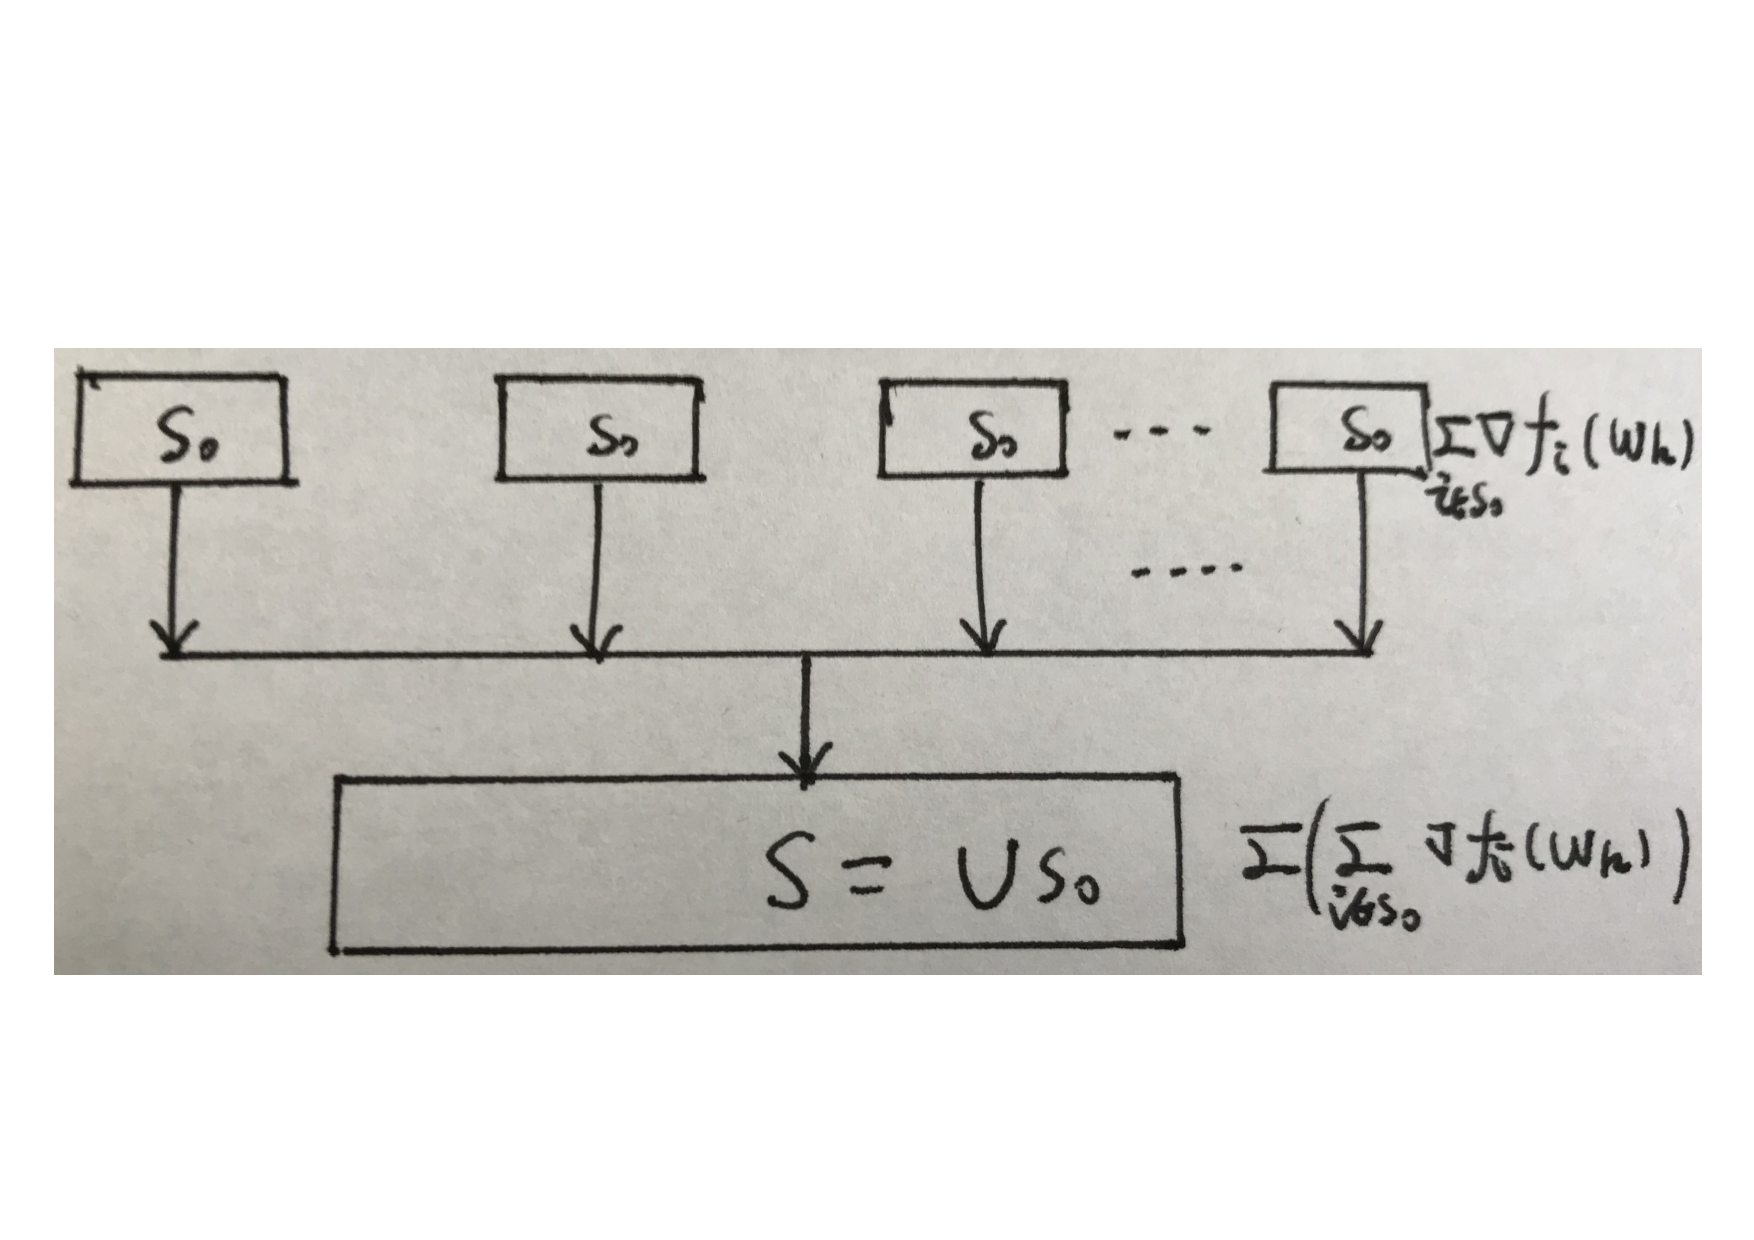
\includegraphics[width=3in]{./figure/FG.pdf}}
\end{center}


\begin{itemize}
  \item 批处理方法在数据集 $\mathbf{S}$ 上优化经验风险 $\rightarrow$ 每次迭代的计算代价将比只在一个 $\mathbf{S}_{\mathrm{sub}}$ 上 计算经验风险要高 10 倍
\end{itemize}

\framebreak

{\color{dblue}实践动机}

对比固定步长的SG 和 L-BFGS 在二分类问题上的性能,目标函数使用 Logistic 损失,使用 RCV1数据集. 
\begin{center}{
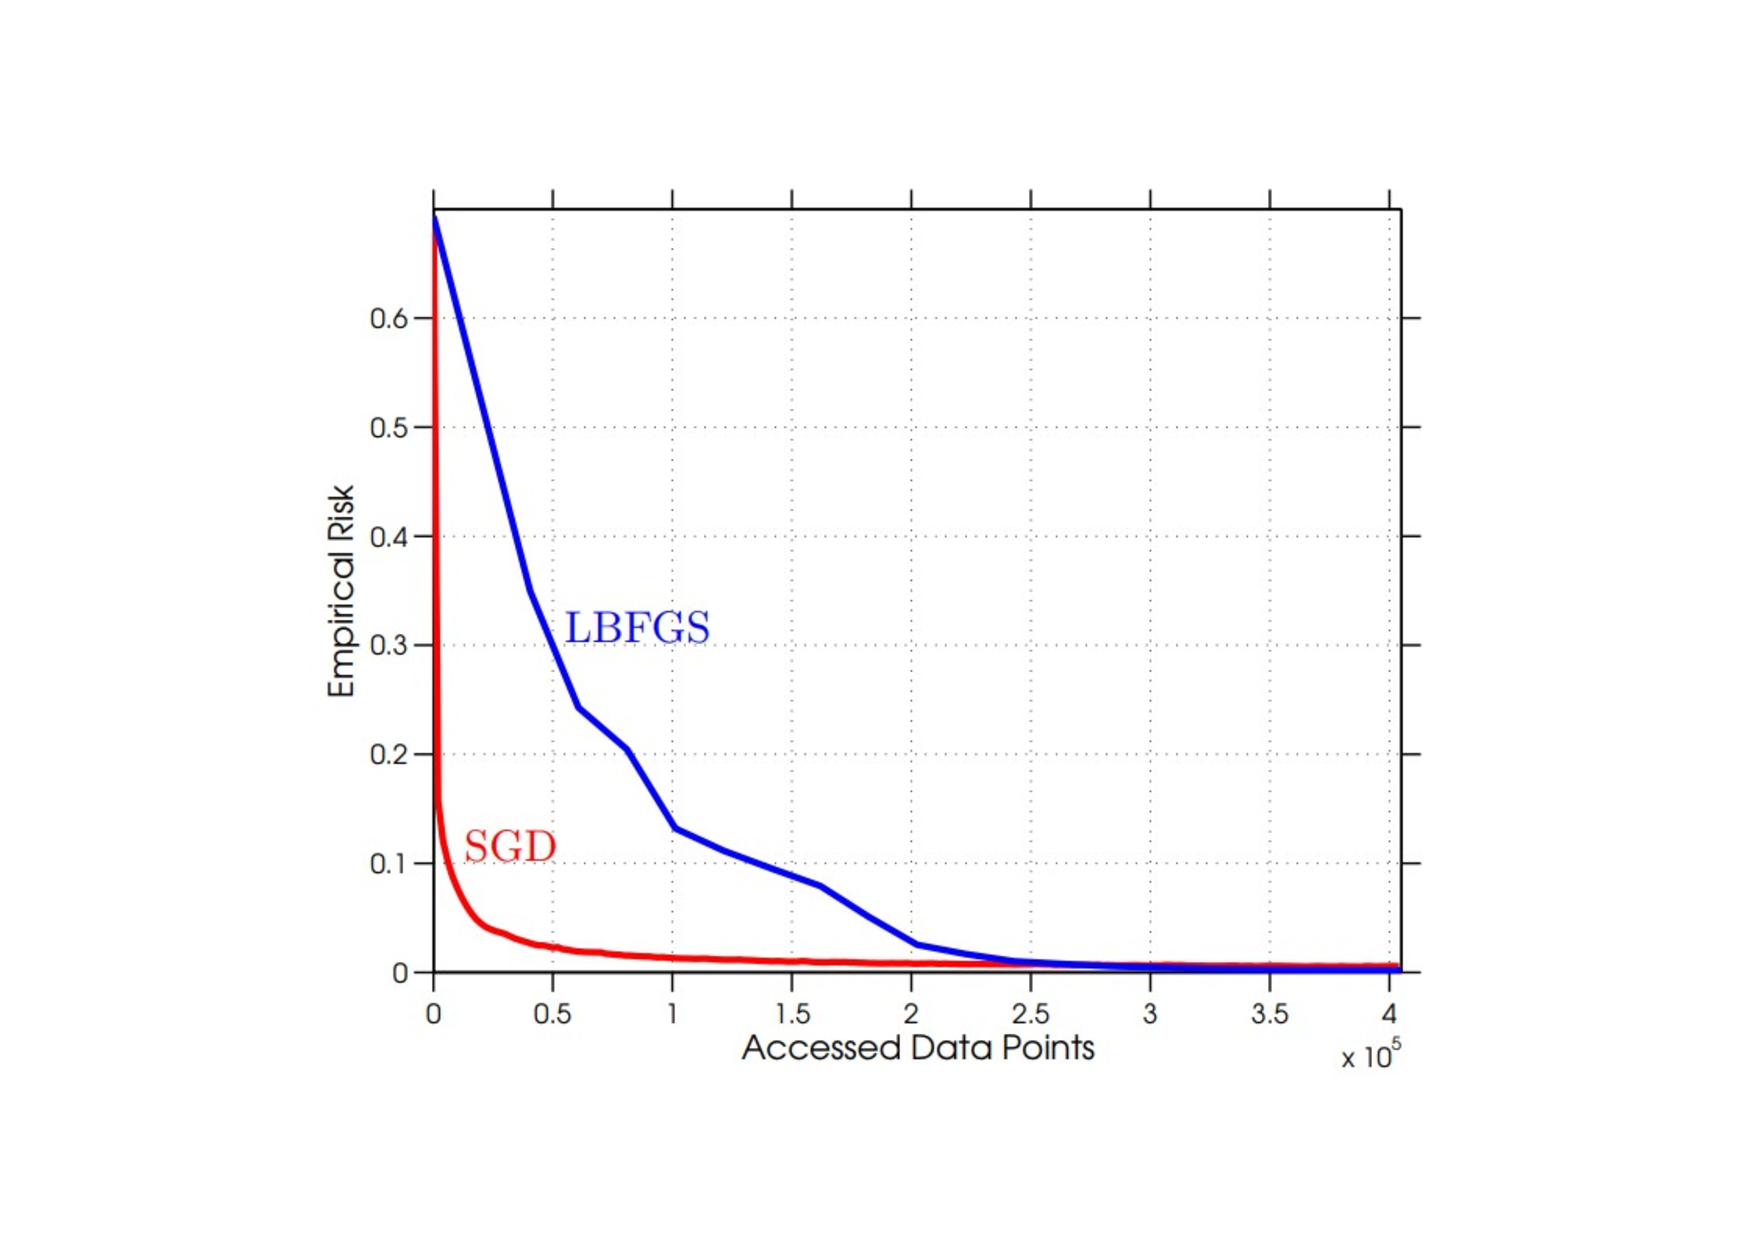
\includegraphics[width=2in]{./figure/SGD-BFGS.pdf}}
\end{center}

\begin{itemize}
  \item[.] SG 在迭代的初始阶段可以\textbf{快速改进}目标函数值
  \item[.] 经过一两个轮次的迭代后,目标函数值改进将\textbf{非常缓慢}
\end{itemize}

\framebreak

{\color{dblue}实践动机}

假设经验风险 $R_n(\boldsymbol{w})=\frac{1}{n} \sum_{i=1}^n f_i(\boldsymbol{w})$ 中
\begin{itemize}
\item[-] 每个 $f_i$ 均是最小值为零的凸二次函数
\item[-] 每个 $f_i$ 的最优解 $\boldsymbol{w}_{i, *}$ 均匀分布在区间 $[0,1]$ 上

% $\rightarrow$ 经验风险 $R_n$ 的最优解为 $\boldsymbol{w}_*=0.5$
\end{itemize}

\bigskip

\begin{center}
%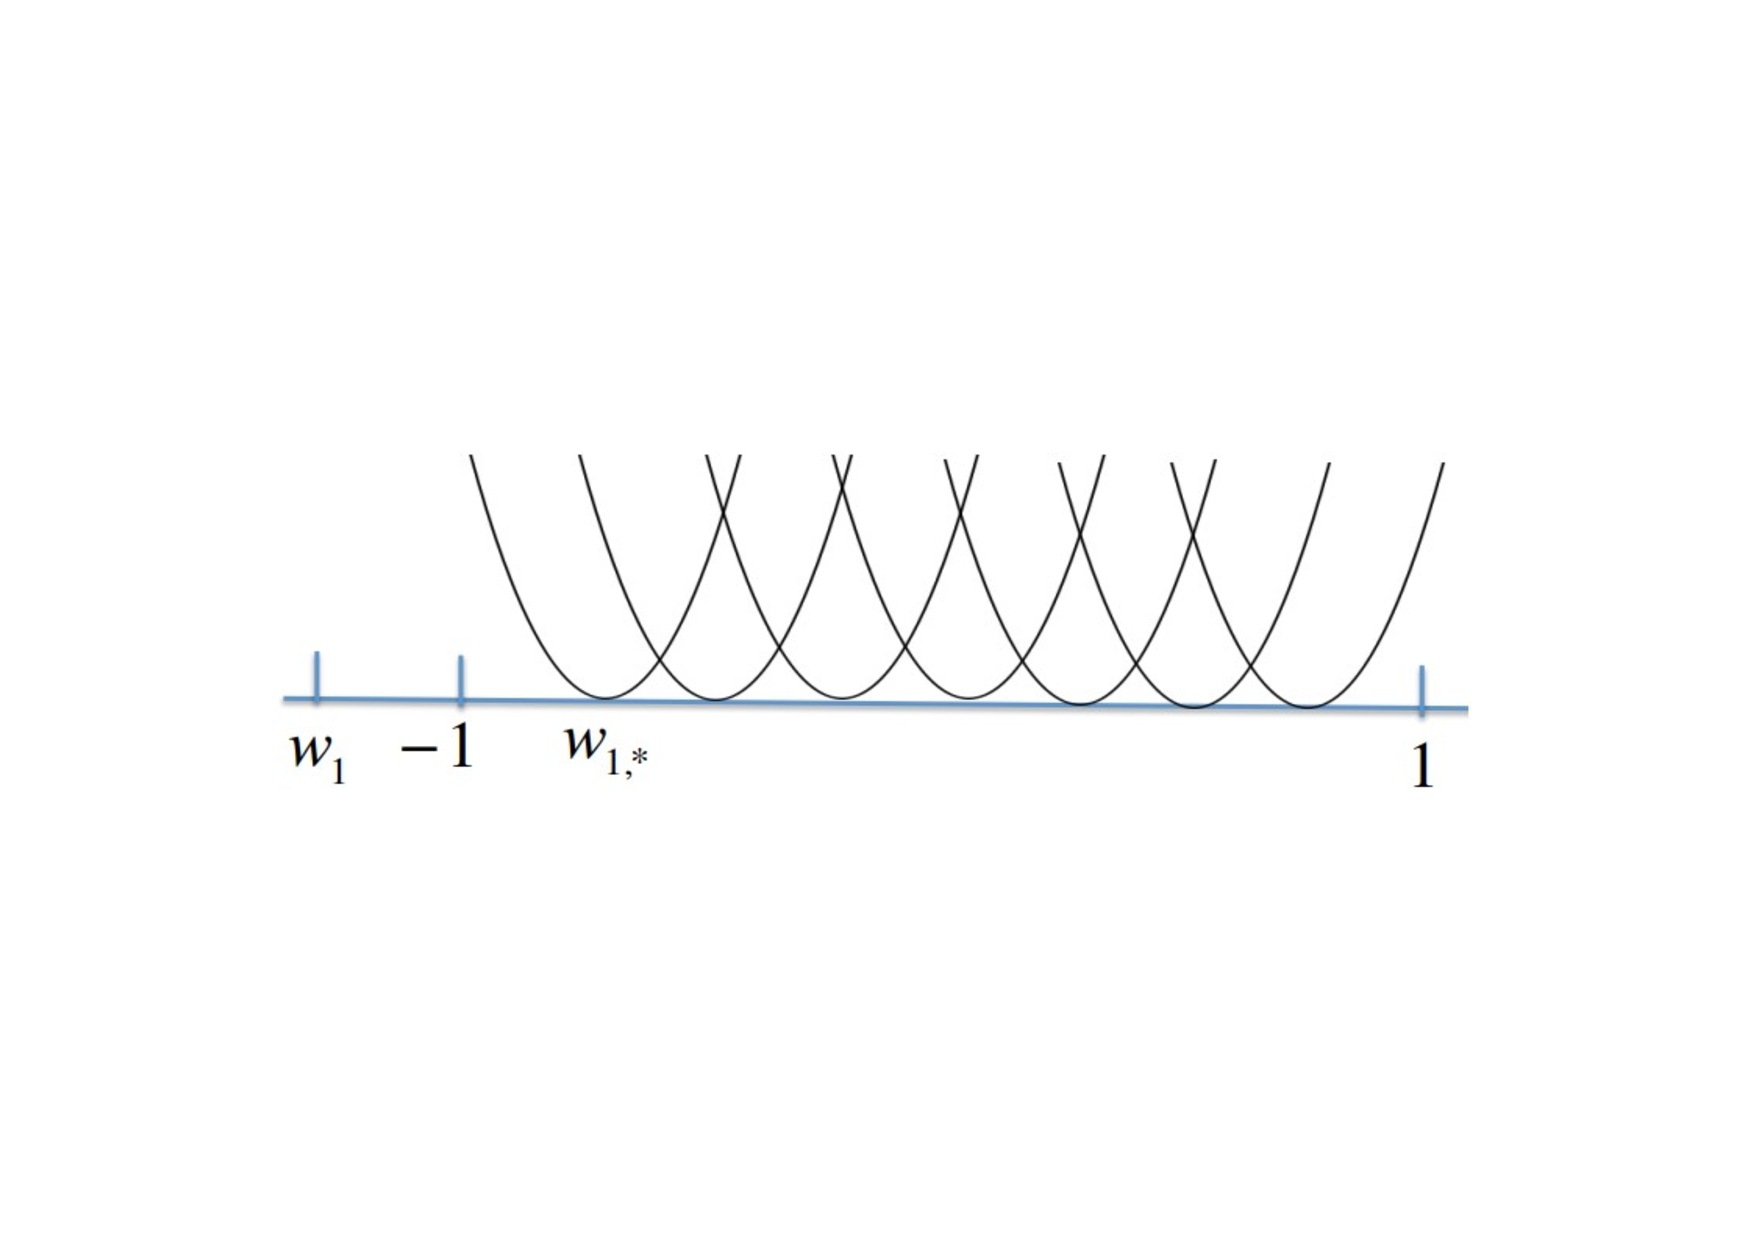
\includegraphics[width=3in, bb=128 217 713 383]{./figure/SG.pdf}}
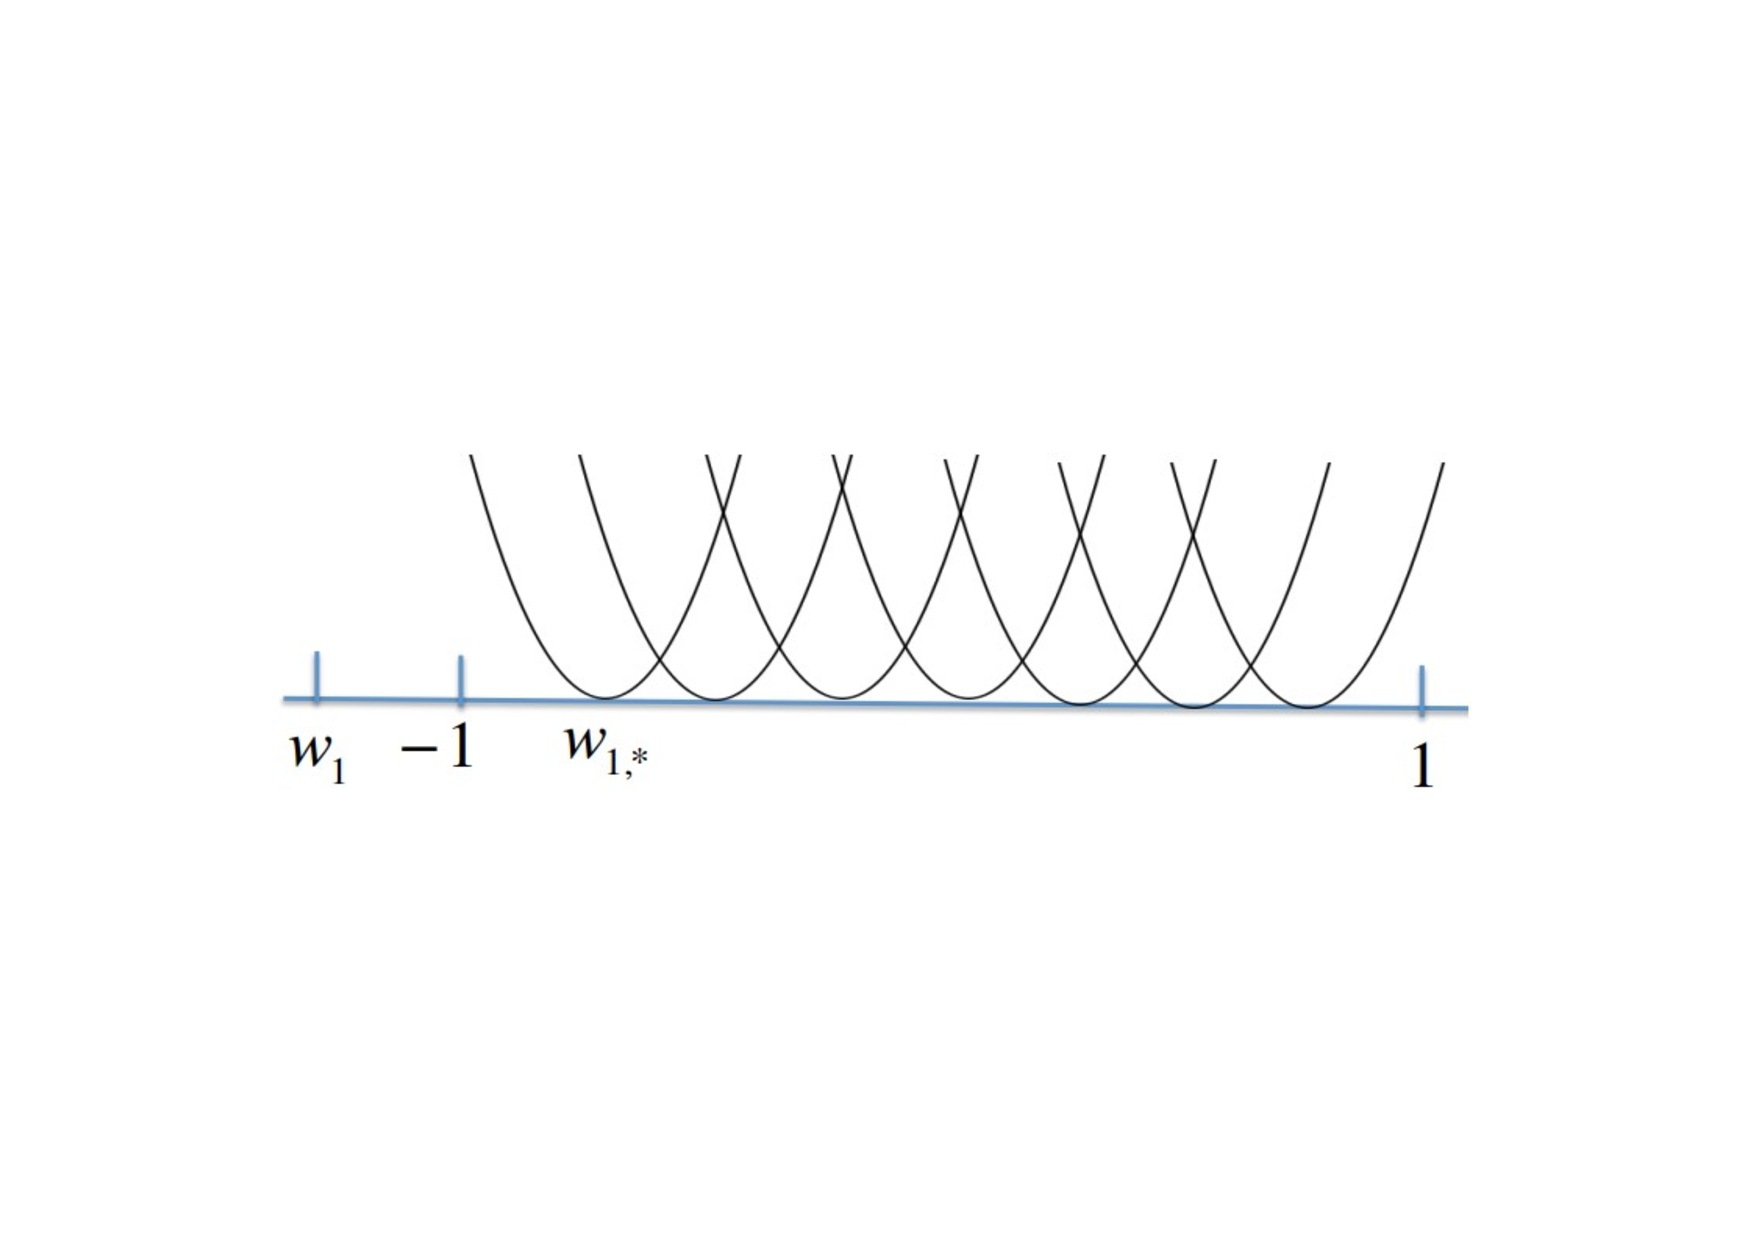
\includegraphics[width=3in]{./figure/SG.pdf}

\end{center}
\framebreak

{\color{dblue}理论动机}

当经验损失 $R_n$ 强凸时$\rightarrow$存在$\rho \in [0,1]$, 对 $k \in \mathbf{N}$都满足

\begin{itemize}
  \item 批处理梯度法
 
$$
  R_n\left(\boldsymbol{w}_k\right)-R_n^* \leqslant O\left(\rho^k\right) \qquad \text{线性收敛}
  $$
  
 
$\Rightarrow$ 求得 $\epsilon$ 最优解所需的计算量与 $n \log \frac{1}{\epsilon}$ 成比例

  \item 随机梯度法
   $$
   \mathbb{E}[F(\mat{w}_k) - F^*] =  \mathcal{O}(\frac{1}{k}) \qquad \text{次线性收敛}
   $$
   $\Rightarrow$  为获得 $\varepsilon$的最优解所需的总计算量与$\frac{1}{\varepsilon}$成正比
\end{itemize}

\textbf{备注:}
\begin{itemize}
  \item[.] 对于不太大的 $n$ 和 $\epsilon$ 值 $\rightarrow$ $\frac{1}{\epsilon}$ 可能大于 $n \log \frac{1}{\epsilon}$ 
  \item[.] 对于$n$很大时(大数据场景) $\rightarrow$ \dred{$n \log(\frac{1}{\varepsilon}) > \frac{1}{\varepsilon}$} 
\end{itemize}
$\Rightarrow$ SG 凭借其更高的计算效率而备受青睐

\end{frame}
%%===========================================================================
\begin{frame}
{小批量随机梯度下降mini-batch SG}

{\color{red}挑战}
\begin{itemize}
\item 经多个轮次迭代后批处理方法的性能可能最终超过随机方法
\item SG 容易陷入局部最小值点或者鞍点
\end{itemize}
$\Rightarrow$ 结合批处理和随机算法的最佳算法 ({\color{dblue}小批量随机梯度下降})

 $$ {\color{red}\mat{w}_{k+1}:=\mat{w}_k-\frac{\alpha_k}{|S_k|}\sum\limits_{i\in S_k}\nabla f_i(\mat{w}_k)}$$

\begin{itemize}
  \item[1.] 降低了参数更新的方差 $\rightarrow$ 收敛更稳定
  \item[2.] 在计算小批量梯度时可以利用一定程度的并行化
\end{itemize}

$\Rightarrow$ 在实践中被广泛使用

\end{frame}

%===========
\section{ SG收敛性分析}


\begin{frame}
{SG 算法伪代码}

\begin{center}

\fbox{
\parbox{0.8\textwidth}{
\begin{center}
\textbf{随机梯度(SG)方法}
\end{center}
\begin{itemize}
\item 选择初始向量 $w_1$
\item  \textbf{for} $k = 1,2,\cdots$ \textbf{do}
\item \qquad 生成   $\xi_k$
\item  \qquad 计算   $g(w_k;\xi_k)$
\item \qquad  选择步长 $\alpha_k>0$
\item  \qquad 迭代更新: $w_{k+1} \leftarrow  w_{k}-\alpha_kg(w_k;\xi_k)$
\item   \textbf{end for}
\end{itemize}
}}\end{center}


\end{frame}



\begin{frame}
\frametitle {SG 算法的收敛性分析}

SG 算法的收敛性主要基于
\begin{itemize}
  \item[i)] 目标函数的\textcolor{red}{光滑化假设}
  \item[ii)] 随机向量$g(w_k;\xi_k)$的\textcolor{red}{一阶矩、二阶矩}假设
\end{itemize}

\bigskip

\textbf{假设 1}:
目标函数 $F$连续可微,且 $F$ 的梯度 Lipschitz连续.
$$\|\nabla F(w) - \nabla F(\overline w)\|_2\leq L\|w - \overline w\|_2 \,\, for \ all\,\, \{w, \overline w\} \subset \mathbb{R}^d.$$

$\rightarrow$ 保证 $F$ 的梯度相对于参数向量的变化率有界

$\Rightarrow$
$$
 F(w) \leqslant F(\overline{w})+\nabla F(\overline{w})^{\mathrm{T}}(w-\overline{w})+\frac{1}{2} L\|w-\overline{w}\|_2^2, \forall w, \overline{w} \subset \mathbb{R}^d
$$

\end{frame}

%===============
\begin{frame}
\frametitle {SG 算法的收敛性分析}

\textbf{假设\,2(一阶矩和二阶矩假设):} 
目标函数和 SG算法满足
\begin{itemize}
  \item[(a)] 迭代序列 $\{w_k\}$ 包含在一个开集中,$F$在开集上有下界 $F_*$.

  \item[(b)] 对于所有的$k$,有$\mu_G \geq \mu > 0$  
  $$\nabla F(w_k)^T \mathbb{E}_{\xi_k}[g(w_k; \xi_k)] \geq \mu\|\nabla F(w_k)\|^2_2 \,\text{且}\,$$
  $$\|\mathbb{E}_{\xi_k}[g(w_k; \xi_k)]\|_2\leq \mu_G\|\nabla F(w_k)\|_2.$$
  \item[(c)] 存在常数$M> 0$ 和 $M_V \geq 0$使得对于所有的 $k$
  $$\mathbb{V}_{\xi_k}[g(w_k; \xi_k)] \leq M + M_V \|\nabla F(w_k)\|^2_2,$$
  其中
  $$\mathbb{V}_{\xi_k}[g(w_k; \xi_k)] := \mathbb{E}_{\xi_k}[\|g(w_k; \xi_k)\|^2_2] - \|\mathbb{E}_{\xi_k}[g(w_k; \xi_k)]\|^2_2.$$
 \end{itemize}

 $\Rightarrow$ 要求$g(w_k, \xi_k)$ 的二阶矩满足
 $$\mathbb{E}_{\xi_k}[\|g(w_k, \xi_k)\|^2_2] \leq M + M_G\|\nabla F(w_k)\|^2_2$$
  其中 $M_G := M_V + \mu^2_G.$
\end{frame}

%%%%%%%%%%%%%%%%%%%%%%%%%%%%%%%%%%%%%%%%%%%%%%%%%%%%%5
\begin{frame}
{\color{dblue}Remarks}
\begin{itemize}
%
\item 假设2(a)仅要求目标函数在算法探索的区域下方有界.

\item 假设2(b)指出,在预期中,向量g是一个足够下降的方向。如果n是F的无偏估计,则它与k立即成立 假设2(b)指出,预期向量 $-g(w_k; \xi_k)$ 是一个合适的下降方向.如果$g(w_k; \xi_k)$是$\nabla F(w_k)$的无偏估计,则它与$\mu_G = \mu = 1$成立 .

\item 对于假设2(c), 记作
$$\mathbb{V}_{\xi_k}[g(w_k, \xi_k)] := \mathbb{E}_{\xi_k}[\|g(w_k,\xi_k)\|^2_2] - \|\mathbb{E}_{\xi_k}[g(w_k, \xi_k)]\|^2_2,$$
它认为
$$\mathbb{E}_{\xi_k}[\|g(w_k, \xi_k)\|^2_2] \leq M + M_G\|\nabla F(w_k)\|^2_2$$
其中 $M_G := M_V + \mu^2_G.$

\end{itemize}
\end{frame}

\begin{frame}
\frametitle {SG 算法的收敛性分析}

\textbf{假设 3(强凸性)} 

目标函数 $F: \mathbf{R}^d \rightarrow \mathbf{R}$ 是强凸的, 即存在常数 $c>0$ 使
$$
F(\overline{\boldsymbol{w}}) \geqslant F(\boldsymbol{w})+\nabla F(\boldsymbol{w})^{\mathrm{T}}(\overline{\boldsymbol{w}}-\boldsymbol{w})+\frac{1}{2} c\|\overline{\boldsymbol{w}}-\boldsymbol{w}\|_2^2, \forall(\overline{\boldsymbol{w}}, \boldsymbol{w}) \in \mathbf{R}^d \times \mathbf{R}^d
$$
由此, $F$ 存在唯一最优值, 记为 $F_*:=F\left(\boldsymbol{w}_*\right)$, 其中 $\boldsymbol{w}_* \in \mathbf{R}^d$

\bigskip

$\rightarrow$ 用目标函数在该点的梯度 $\ell_2$ 范数的平方来估计最优间隙的界
$$
2 c\left(F(\boldsymbol{w})-F_*\right) \leqslant\|\nabla F(\boldsymbol{w})\|_2^2, w \in \mathbf{R}^d
$$

\end{frame}


%===================
\begin{frame}
\frametitle {SG 算法的收敛性分析}

% {\color{dblue}{强凸目标函数, 固定步长}}

\begin{theorem}[\color{dblue}{强凸目标函数, 固定步长}]

在假设 1-3 成立的条件下, 记 $F_*$ 为目标 函数的最优值, 对于所有 $k \in \mathbf{N}$, 设步长 $\alpha_k=\bar{\alpha}$ 满足
\begin{equation}\label{4.13}
0<\bar{\alpha} \leqslant \frac{\mu}{L M_G}
\end{equation}
则对所有的 $k \in \mathbf{N}$, 最优间隙的期望满足以下不等式:
\begin{equation}\label{4.14}
E\left[F\left(\boldsymbol{w}_k\right)-F_*\right] \leqslant \frac{\bar{\alpha} L M}{2 c \mu}+(1-\bar{\alpha} c \mu)^{k-1}\left(F\left(\boldsymbol{w}_1\right)-F_*-\frac{\bar{\alpha} L M}{2 c \mu}\right) \stackrel{k \rightarrow \infty}{\longrightarrow} \frac{\bar{\alpha} L M}{2 c \mu}
\end{equation}

\end{theorem}

\begin{itemize}

  \item 如果 $g(w_k;\xi_k)$ 是\textbf{无偏估计} $\rightarrow$ $\mu = 1$
  \item 且如果$g(w_k;\xi_k)$ 中\textbf{没有噪声} 

  $\rightarrow$  可假设$M_G = 1$, 
  简化为$\alpha\in (0,\frac{1}{L})$(FG经典步长要求)
\end{itemize}
%
\end{frame}
%==========

\begin{frame}
\frametitle {SG 算法的收敛性分析}


\begin{itemize}
  \item
 在Robbins和Monro的开创性作品中,步长采用:
$$\sum\limits_{i=1}^{\infty}\alpha_k=\infty, \sum\limits_{i=1}^{\infty}\alpha_k^2<\infty.$$
\end{itemize}

\begin{theorem}[{\color{dblue}{强凸性,步长递减}}]
在假设 1-3成立的条件下 SG方法的步长满足
$$\alpha_k=\frac{\beta}{\gamma+k}\text{\,对于 \,}\beta>\frac{1}{c\mu}\,\text{且}\,
 \gamma>0\,\text{使其满足}\,\, \alpha_1\leq\frac{c}{L M_G}.$$
那么,
$$\mathbb{E}[F(w_k)-F_*]\leq \frac{\nu}{\gamma+k}.$$
其中
$$\nu:= \max\left\{\frac{\beta^2L M}{2(\beta c\mu-1)}, (\gamma+1)(F(w_1)-F_*)\right\}.$$

\end{theorem}
\end{frame}


\begin{frame}
\frametitle{  降噪方法}

梯度估计中的噪声会阻止目标函数值的收敛
\begin{itemize}
\item 在固定步长下的解决方案
 $\mathbb{E}[F(w_k)-F_*] \stackrel{K\rightarrow\infty}{\leq} \frac{\bar{\alpha}LM}{2c\mu}$

 %    $\bar{\alpha}$
\item 步长递减序列下的次线性收敛速度
\end{itemize}
\end{frame}

\begin{frame}
\frametitle{降噪方法}
开发{\textcolor{blue}{具有降噪能力}}的方法
\begin{itemize}
\item 动态采样方法:逐渐增加梯度计算中使用的小批量大小
\item 梯度聚合方法:通过存储与先前迭代中使用的样本相对应的梯度估计, {\color{dblue}提高搜索方向的质量}
\item 迭代平均方法:在优化过程中保持迭代$w_k$的平均值
\end{itemize}
\end{frame}

%===========================
\section{梯度聚合}

\begin{frame}
\frametitle{降噪-梯度聚合方法}

{\color{red}\textbf{Q: }是否可以通过重复使用或修改先前计算的信息来降低方差?}

\begin{itemize}
\item 如果当前迭代没有与以前的迭代相距较大$\rightarrow$来自以前迭代的随机梯度信息可能仍然有用

\item 如果在存储中保持索引梯度估计$\rightarrow$可以在收集新信息时修改特定的估计
\end{itemize}

\bigskip

$\Rightarrow$ {\color{dblue}梯度聚合}的概念,如SVRG (随机方差约减梯度)、SAGA(随机平均梯度算法)
\end{frame}


%===============
\begin{frame}[fragile]
  \frametitle{SVRG (随机方差约减梯度)}

  \textbf{SVRG属于循环法}

  在每个循环的开始有一个初始值 $\boldsymbol{w}_k$, 并计算出一个批量梯度 
  $$
  \nabla R_n\left(\boldsymbol{w}_k\right)=\frac{1}{n} \sum_{i=1}^n \nabla f_i\left(\boldsymbol{w}_k\right),
  $$
   并初始化 $\tilde{\boldsymbol{w}}_1 \leftarrow \boldsymbol{w}_k$, 然后执行一组由 $j$ 作为索 引的 $m$ 次内部迭代更新 $\tilde{\boldsymbol{w}}_{j+1} \leftarrow \tilde{\boldsymbol{w}}_j-\alpha \tilde{\boldsymbol{g}}_j$, 其中
  $$
  \tilde{\boldsymbol{g}}_j \leftarrow \nabla f_{i_j}\left(\tilde{\boldsymbol{w}}_j\right)-\left(\nabla f_{i_j}\left(\boldsymbol{w}_k\right)-\nabla R_n\left(\boldsymbol{w}_k\right)\right)
  $$
  $i_j \in\{1, \cdots, n\}$ 是随机选择的指标

  \bigskip

  $\bullet$ 关于$\tilde{\boldsymbol{g}}_j \leftarrow \nabla f_{i_j}\left(\tilde{\boldsymbol{w}}_j\right)-\left(\nabla f_{i_j}\left(\boldsymbol{w}_k\right)-\nabla R_n\left(\boldsymbol{w}_k\right)\right)$的简单解释:
   \begin{itemize}
      \item[-]  $\bbe_{i_j} \nabla f_{i_{j}}\left(w_{k}\right) = \nabla R_{n}\left(w_{k}\right)$\\
      % $\rightarrow$ 每次迭代随机抽取一个样本点并计算当前迭代 $\tilde{w}_j$ 处的随机梯度 $\nabla f_{i_j}\left(\tilde{\boldsymbol{w}}_j\right)$, 并根据预估的偏差对其进行修正
      %%\item $\nabla f_{i_{j}}\left(w_{k}\right)-\nabla R_{n}\left(w_{k}\right)$:   bias in the gradient estimate $\nabla f_{i_{j}}\left(w_{k}\right).$
      \item[-] $\tilde{g}_{j}$ 代表了 $\nabla R_{n}\left(\tilde{w}_{j}\right)$ 的一个无偏估计量,但其方差预期会比简单选择SG ($\tilde{g}_{j}=\nabla f_{i_{j}}\left(\tilde{w}_{j}\right)$)小很多
      
  \end{itemize}

  
\end{frame}

\begin{frame}
% \frametitle{SVRG (随机方差约减梯度)}
\begin{center}
\fbox{
\parbox{0.8\textwidth}{
\begin{center}
\textbf{  最小化 $R_n$的SVRG方法}
\end{center}

初始值 $w_1 \in \mathbb{R}^d$, 步长 $\alpha> 0$,  $m$次迭代

\textbf{for} $k=1,2,\cdots, $ \textbf{do}\\
\hspace{1em} 计算出一个批量梯度 $\nabla R_n(w_k)$\\
\ \ \ 初始化 $\tilde{w}_{1} \leftarrow w_{k}$\\
\ \ \ \textbf{for} $j=1,2,\cdots,m $ \textbf{do}\\
       从 $\{1,\cdots,n\}$ 随机选择 $i_j$ \\
\ \ \ \ \  $\tilde{g}_{j} \leftarrow \nabla f_{i_{j}}\left(\tilde{w}_{j}\right)-\left(\nabla f_{i_{j}}\left(w_{k}\right)-\nabla R_{n}\left(w_{k}\right)\right)$\\
 $\tilde{w}_{j+1} \leftarrow \tilde{w}_{j}-\alpha \tilde{g}_{j}$\\
\textbf{end for}\\
选项 (a): 取 $w_{k+1}=\tilde{w}_{m+1}$\\
选项 (b): 取 $w_{k+1}=\frac{1}{m} \sum_{j=1}^{m} \tilde{w}_{j+1}$\\
选项 (c): 从$1,\cdots,m$选择$j$  ,取 $w_{k+1}=\tilde{w}_{j+1}$\\
\textbf{end for}
}}
\end{center}
\end{frame}

%=================
\begin{frame}
\frametitle{SVRG (随机方差约减梯度)}


对于选项 (b) 和 (c), 在最小化强凸目标 $R_n$ 时, 算法可以实现\textbf{线性收敛速度}。
选择合适的步长 $\alpha$ 和内循环次数 $m$, 使下式
$$
\rho:=\frac{1}{1-2 \alpha L}\left(\frac{1}{m c \alpha}+2 L \alpha\right)<1,
$$
并假设算法的当前迭代点为 $\boldsymbol{w}_k$, 那么, 有如下不等式成立
$$
\mathbb{E}\left[R_n\left(\boldsymbol{w}_{k+1}\right)-R_n\left(\boldsymbol{w}_*\right)\right] \leqslant \rho \mathbb{E}\left[R_n\left(\boldsymbol{w}_k\right)-R_n\left(\boldsymbol{w}_*\right)\right]
$$
其中, 期望是对内循环中的随机变量取的。

\bigskip

\begin{footnoteremark}
这里得到的线性收敛率适用于外部迭代点列$\{w_k\}$,其中
\begin{itemize}
  \item[.] 从$w_k$ 到$w_{k+1}$的每一步需要计算 $2m + n$ 个样本梯度
  % \item[.] 第 7 步需要计算 2 次随机梯度
  % \item[.] 第 3 步需要计算全梯度
\end{itemize}
$\Rightarrow$  SVRG 的一次迭代比 SG 的一次迭代的计算量 要多得多, 实际上与全梯度方法一次迭代的计算量相当

\end{footnoteremark}

\end{frame}

%=========================
\begin{frame}
\frametitle{SVRG (随机方差约减梯度)}

\textbf{\color{dblue}与SG对比}

\begin{figure}
  \centering
  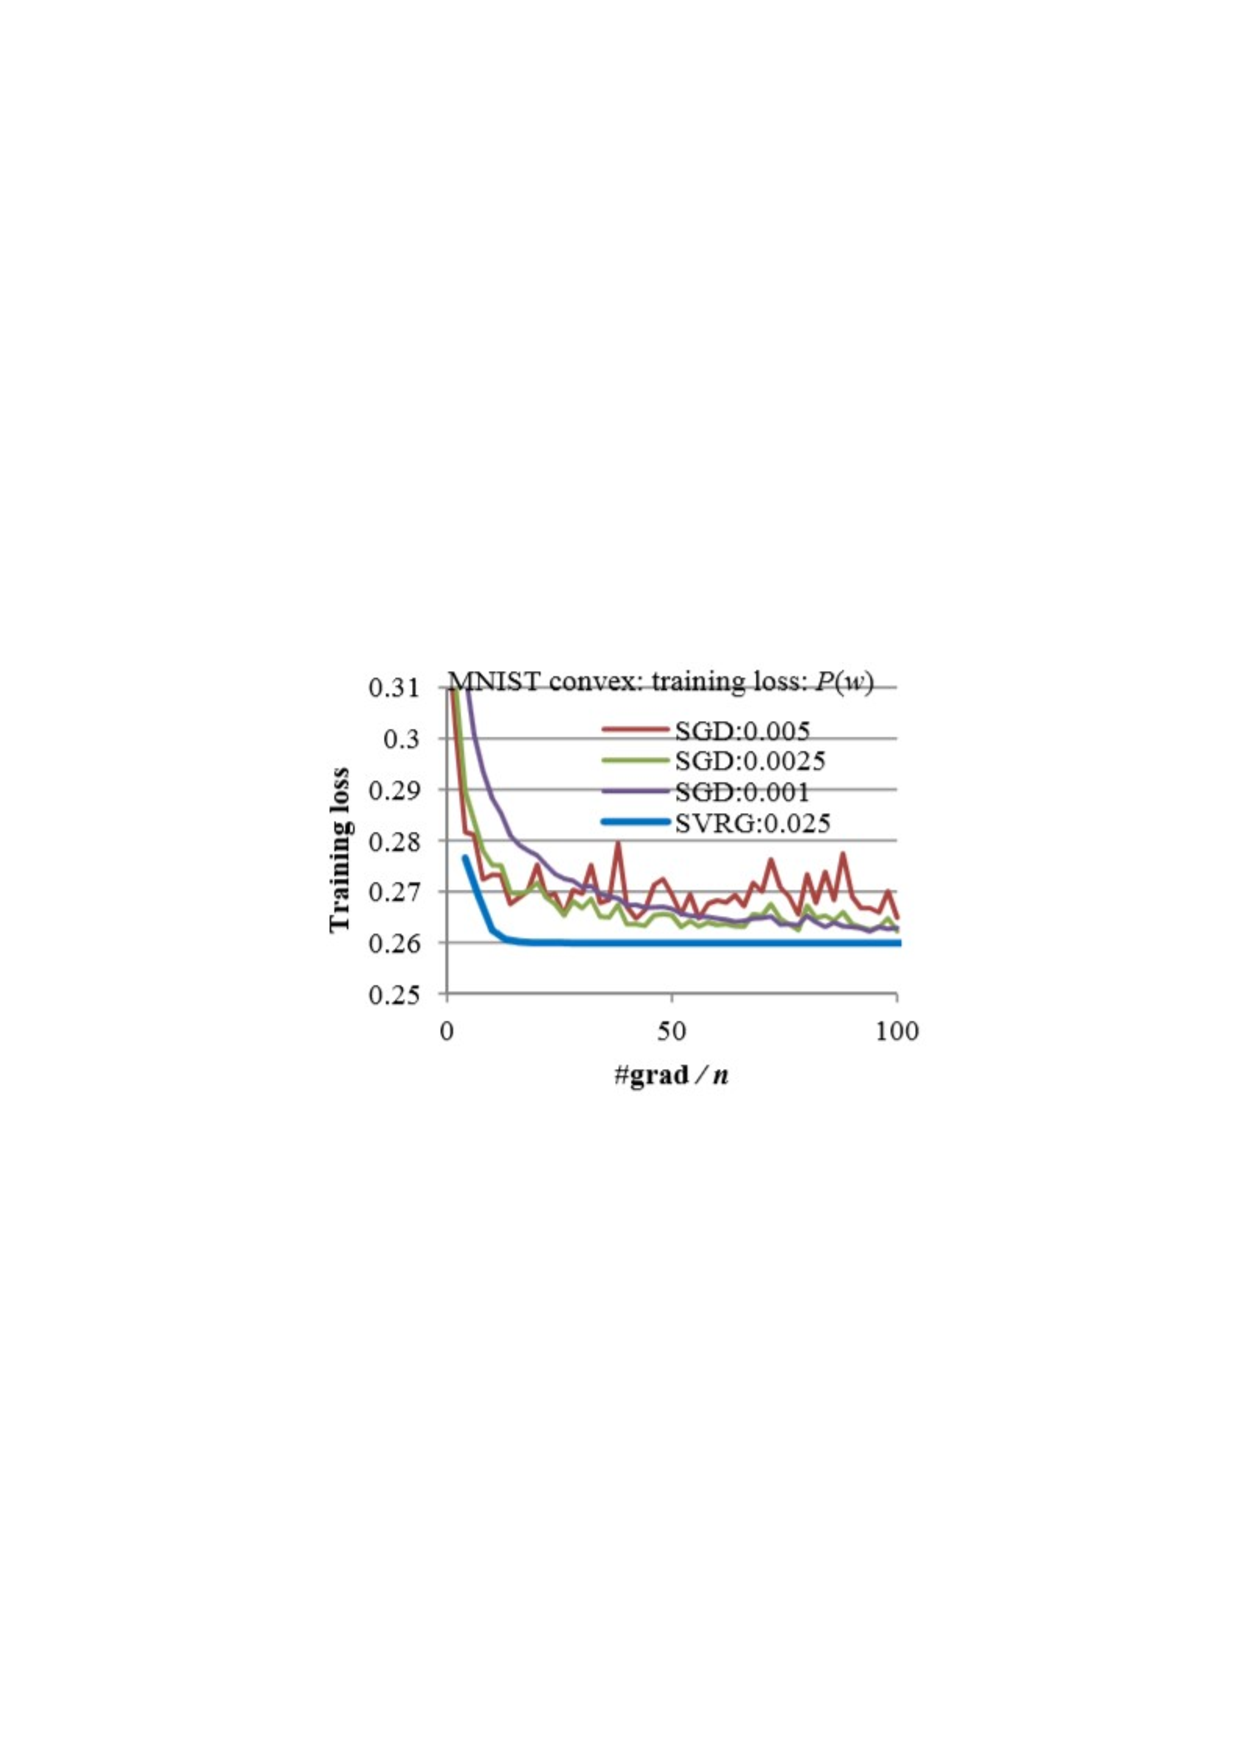
\includegraphics[width=2.3in ]{./figure/SVRG.pdf}\\
%  \caption{}\label{}
\end{figure}
\begin{itemize}
\item
在实践中,如果需要高训练精度,则与SG相比,SVRG在某些应用中似乎非常有效.


\end{itemize}
\end{frame}



\begin{frame}[fragile]
  \frametitle{SAGA(随机平均梯度算法)}

SAGA 方法 不涉及周期性操作, 除在初始点以外无需计算全梯度

在每次迭代中, 它计算一个随机向量 $\boldsymbol{g}_k$ 
\begin{itemize}
  \item 存储目标函数中各 $f_i$ 在某迭代点的梯度 $\nabla f_i\left(\boldsymbol{w}_{[i]}\right)$
  \begin{itemize}
  \item[.]  其中 $\boldsymbol{w}_{[i]}$ 表示最近一次计算 $f_i$ 的梯度时使用的迭代点
  \end{itemize}
  \item 在第 $k$ 个迭代步, 随机选择一个整数 $j \in\{1, \cdots, n\}$, 计算 $\boldsymbol{g}_k$
  $$
  \boldsymbol{g}_k \leftarrow \nabla f_j\left(\boldsymbol{w}_k\right)-\nabla f_j\left(\boldsymbol{w}_{[j]}\right)+\frac{1}{n} \sum_{i=1}^n \nabla f_i\left(\boldsymbol{w}_{[i]}\right)
  $$
\end{itemize}
 
  \bigskip

  若将 $\boldsymbol{g}_k$ 关于 $j \in\{1, \cdots, n\}$ 取期望, 则有 $\mathbb{E}\left[\boldsymbol{g}_k\right]=\nabla R_n\left(\boldsymbol{w}_k\right)$

  $\Rightarrow$ SAGA计算的随机向量是梯度的无偏估计, 但其方差小于基本 SG 算法所产生的方差

\end{frame}

\begin{frame}
\begin{center}
\fbox{
\parbox{0.8\textwidth}{
\begin{center}
\textbf{  最小化 $R_n$的SARA方法}
\end{center}

选择一个初始值 $\boldsymbol{w}_1 \in \mathbf{R}^d$, 步长 $\alpha>0$\\
\textbf{for}  $i \in\{1, \cdots, n\}$ \textbf{do}\\
\hspace{1em}  计算梯度 $\nabla f_i\left(\boldsymbol{w}_1\right)$\\
\ \ \  储存 $\nabla f_i\left(\boldsymbol{w}_{[i]}\right) \leftarrow \nabla f_i\left(\boldsymbol{w}_1\right)$ \\
\textbf{end for}\\
\textbf{for} $k=1,2, \cdots$ \textbf{do}\\
\hspace{1em} 从 $\{1, \cdots, n\}$ 中随机选择一个整数 $j$\\
\ \ \  计算梯度 $\nabla f_j\left(\boldsymbol{w}_k\right)$\\
\ \ \ 令 $\boldsymbol{g}_k \leftarrow \nabla f_j\left(\boldsymbol{w}_k\right)-\nabla f_j\left(\boldsymbol{w}_{[j]}\right)+\frac{1}{n} \sum_{i=1}^n \nabla f_i\left(\boldsymbol{w}_{[i]}\right)$\\
\ \ \  储存 $\nabla f_j\left(\boldsymbol{w}_{[j]}\right) \leftarrow \nabla f_j\left(\boldsymbol{w}_k\right)$\\
\ \ \  令 $\boldsymbol{w}_{k+1} \leftarrow \boldsymbol{w}_k-\alpha \boldsymbol{g}_k$\\
\textbf{end for}\\

}}
\end{center}
\end{frame}


\begin{frame}[fragile]
  \frametitle{SAGA(随机平均梯度算法)}
   当最小化强凸$R_{n}$时,该方法可以实现线性收敛速度

   具体来说,取 $\alpha=1 /(2(c n+L))$, 可得如下估计
  $$
  \begin{aligned}
    \mathbb{E}\left[\left\|w_{k}-w_{*}\right\|_{2}^{2}\right] & \leq\left(1-\frac{c}{2(c n+L)}\right)^{k}\left(\left\|w_{1}-w_{*}\right\|_{2}^{2}+\frac{n D}{c n+L}\right) \\
    \text { 其中 } D: &=R_{n}\left(w_{1}\right)-\nabla R_{n}\left(w_{*}\right)^{T}\left(w_{1}-w_{*}\right)-R_{n}\left(w_{*}\right)
  \end{aligned}
  $$
\end{frame}

\begin{frame}[fragile]
  \frametitle{SG vs 梯度聚合方法}
\hint{尽管本小节中所介绍的梯度聚合方法比 SG 具有更快的收敛速度,这并不能表明它们明
  显优于 SG}
\begin{itemize}
  \item SG 的计算时间为 $$T(n, \epsilon) \sim \kappa^{2} / \epsilon$$ 
  其中 $\kappa:=L / c$
  \item SVRG和SAGA 的计算时间为
  $$\mathcal{T}(n, \epsilon) \sim(n+\kappa) \log (1 / \epsilon)$$

  随着样本点数量$n$的增加而增加
\end{itemize}

$\Rightarrow$
\begin{itemize}
  \item[*] 对于非常大的$n$,梯度聚合方法的时间复杂度与批处理相似
  \item[*] 如果 $\kappa$ 接近 1 , 那么 $SG $ 显然会更有效
  \item[*] 当 $\kappa \gg n$时, 梯度聚合方法会表现的更好
\end{itemize}
\end{frame}


%========================================

\section{二阶方法}
\begin{frame}[fragile]
	\frametitle{二阶方法}
	\normaltitle{动机}
	\begin{itemize}
		\item 一阶方法,例如SG和全梯度法,它们\textit{不是尺度不变的}.
		\item 一阶方法的每次迭代通过计算目标函数的二阶泰勒近似的极小值点作为后续迭代点.
		\item 目标函数的高度非线性和病态条件的不利影响.
	\end{itemize}
	
\end{frame}





%===========================================================================================================
%===========================================================================================================
\begin{frame}[allowframebreaks]%119
\frametitle{二阶方法的动机}
%\footnotesize{}
%In section\,5, we looked beyond classical SG to methods that are less affected by noise in the stochastic  directions.
%Another manner in which one can move beyond classical SG is to address the averse effects of high nonlinearity
%and ill-conditioning of the objective function through  the use of second-order information.

{\normalsize\textbf{动机 .}}

 \dblue{尺度不变}:

 * 考虑最小化连续可微函数  $F: R^d \rightarrow
R$,
\begin{equation}\label{EQ_6_1}
    w_{k+1} \leftarrow w_k - \alpha_k \nabla F(w_k).
\end{equation}

* 交替迭代:
$$
\dblue{
    \min_{\bar{w}}\ F(B\bar{w})
}
$$
假设 $B$为对称正定矩阵.
全梯度迭代格式:
$$
    \bar{w}_{k+1} \leftarrow \bar{w}_k - \alpha_k B \nabla F(B\bar{w}_k),
$$
两端乘以 $B$并由定义\dblue{$w_k = B \bar{w}_k$}, 可得如下迭代
\begin{equation}\label{EQ_6_2}
    w_{k+1} \leftarrow w_k - \alpha_k \dblue{B^2} \nabla F(w_k).
\end{equation}

对比(\ref{EQ_6_1}) 和 (\ref{EQ_6_2}):
\begin{itemize}
    \item 在这种尺度变化的情况下,算法的表现会有所不同.

     \item  例如, 当$F$是具有唯一极小值$w_*$的强凸二次函数时,

       (\ref{EQ_6_1}): 通常需要多次迭代才能逼近极小值

       (\ref{EQ_6_2}): 只需要一步的迭代 $B = (\nabla^2F(w_k))_{}^{-1/2}$, $\alpha = 1$.

         (牛顿方法的一次迭代).

\end{itemize}
\end{frame}


\begin{frame}[allowframebreaks]
\frametitle{高斯-牛顿方法}

介绍

\begin{itemize}
\item
 \dblue{非线性最小二乘法的经典方法,} 即最小化问题,其中目标函数是平方和。

\item  这个想法也适用于其他流行的损失函数。

\item
\dblue{优点}:  它仅使用保证是半正定的一阶信息来构造对Hessian的近似,

\item
\dblue{限制:} %it ignores second-order interactions between elements of the parameter $w$.
忽略(一般)损失函数 $\ell$的曲率.
\end{itemize}

\framebreak

输入输出对 $\xi:=(x,y)$,
由参数向量$w$ 引起的损失是在$h(x;w)\in R^d$ 和 $y \in R^d$之间测量的:
 %via a squared norm discrepancy:
%%Representing the input-output pair being chosen randomly via the subscript $\xi$, we may thus write
$$
    f(w,\xi) = \ell(h(x_{\xi};w),y_{\xi}) = \frac{1}{2} \|h(x_{\xi};w) - y_{\xi}\|_2^2
    = \frac{1}{2} \sum_{i=1}^N (h(x_{\xi_i};w) - y_{\xi_i})^2.
$$

\begin{itemize}
\item 牛顿迭代:$f(w,\xi)$在$w_k$附近的二阶泰勒级数模型

\item 高斯-牛顿迭代:对二次损失函数内的预测函数$h$进行仿射近似。
\end{itemize}

\end{frame}

\begin{frame}[allowframebreaks]
\frametitle{高斯-牛顿迭代}


 $J_h(\cdot;\xi)$:  $h(x_{\xi}; \cdot)$相对于$w$的雅可比

$$
    h(x_{\xi};w) \approx h(x_{\xi};w_k) + J_h(w_k;\xi)(w-w_k),
$$
这导致
$$
    \begin{aligned}
        f(w;\xi) & \approx \frac{1}{2} \| h(x_{\xi};w_k) + J_h(w_k;\xi)(w-w_k) - y_{\xi}^{}\|_2^2 \\
            & =  \frac{1}{2} \| h(x_{\xi};w_k)- y_{\xi}^{}\|_2^2 +    (h(x_{\xi};w_k)- y_{\xi}^{})_{}^{T} J_h(w_k;\xi)(w-w_k)\\
    \end{aligned}
$$

\begin{flushright}
  $ +     \dblue{  \frac{1}{2}(w-w_k) J_h(w_k;\xi)^{T}  J_h(w_k;\xi)(w-w_k)}.$
\end{flushright}

\bigskip
\textbf{高斯-牛顿矩阵}

  \dblue{用高斯-牛顿矩阵替换次采样的Hessian矩阵 }%(\ref{EQ_6_5})  
 \begin{equation}\label{EQ_6_15}
G_{S_k^H}(w_k; \xi_k^H) = \frac{1}{|S_k^H|} \sum_{i\in S_k^H} J_h(w_k;\xi_{k,i})^{T}  J_h(w_k;\xi_{k,i}).
\end{equation}

\breakframe

\textbf{比较高斯-牛顿近似和牛顿近似}


$$   f(w,\xi) = \ell(h(x_{\xi};w),y_{\xi}) = \frac{1}{2} \|h(x_{\xi};w) - y_{\xi}\|_2^2 = \sum_{i=1}^N (h(x_{\xi_i};w) - y_{\xi_i})^2.
 $$

$f(w,\xi)$ 在 $w = w_k$的泰勒展开式:

\begin{small}
    $$    f(w,\xi) \approx
        f(w_k,\xi) + \langle \nabla_w f(w_k,\xi), w-w_k\rangle
            + \frac{1}{2} (w-w_k)^T \nabla_w^2 f(w_k,\xi)\cdot(w-w_k),  $$
\end{small}
\bigskip

$    \nabla_w f(w_k,\xi) =     \nabla_w h(x_{\xi},w_k) \cdot ( h(x_{\xi},w_k)-y_{\xi})= $

\rightline{
$            \dblue{
        \left[\nabla_w h(x_{\xi_1},w_k),\cdots,\nabla_w h(x_{\xi_N},w_k) \right] }
              \cdot
                \left[\begin{array}{c}
                  h(x_{\xi_1},w_k)-y_{\xi_1}  \\
                  \cdots \\
                  h(x_{\xi_N},w_k)-y_{\xi_N}  \\
                \end{array}\right],               $
}

$  \nabla_w^2 f(w_k,\xi)=\sum_{i=1}^N\nabla_w h(x_{\xi_i},w_k) \cdot \nabla_w h(x_{\xi_i},w_k)^T$
\begin{flushright}
  $\dblue{ + \sum_{i=1}^N \nabla_w^2 h(x_{\xi_i},w_k)  \cdot (h(x_{\xi_i},w_k)-y_{\xi_i}).} $
\end{flushright}


\end{frame}
%===========================================================================================================
%===========================================================================================================

\begin{frame}
{高斯-牛顿矩阵的奇异问题}

\begin{itemize}
\item \dblue{挑战.}
 高斯-牛顿矩阵通常是奇异的或近似奇异的.

\item \dblue{解决.}
%In practice, this is typically handled by
通过向其添加单位矩阵的正倍数来正则化.

\item \dblue{应用.}
%For least squares loss functions,
不精确的Hessian自由牛顿方法和具有如(\ref{EQ_6_14})中定义的梯度位移向量的随机拟牛顿方法可以应用(正则化的)高斯-牛顿近似:保证是正定的.
\end{itemize}
\end{frame}

%===========================================================================================================

\begin{frame}
{广义高斯-牛顿法}


$$
    f(w,\xi) = \ell(h(x_{\xi};w),y_{\xi})
    = \frac{1}{2} \sum_{i=1}^N \ell(h(x_{\xi_i};w) - y_{\xi_i}).
$$

 预测函数的仿射逼近 $h(x_{\xi};w)$ $+$ 损失函数的二阶泰勒展开式 $l$ $\longrightarrow$  广义高斯-牛顿矩阵
\begin{equation}\label{EQ_6_16}
G_{S_k^H}(w_k; \xi_k^H) = \frac{1}{|S_k^H|} \sum_{i\in S_k^H} J_h(w_k;\xi_{k,i})^{T} \dblue{H_l(w_k;\xi_{k,i})}J_h(w_k;\xi_{k,i}).
\end{equation}
其中 $H_l(w_k;\xi) = \frac{\partial^2 l }{\partial h^2}(h(x_{\xi}; w_k),y_k)$
捕获损失函数的曲率 $l$. * 它是 (\ref{EQ_6_15}) 的推广,其中 $H_l = I$.
\end{frame}

\begin{frame}
{广义高斯-牛顿法}

训练DNN时,
 使用形式为 
\dblue{$f(w;\xi) = -\log (h(x_{\xi};w))$} 的对数损失

广义高斯-牛顿矩阵:
\begin{equation}\label{EQ_6_17}
\begin{aligned}
G_{S_k^H}(w_k; \xi_k^H) & = \frac{1}{|S_k^H|} \sum_{i\in S_k^H} J_h(w_k;\xi_{k,i})^{T} \dblue{\frac{1}{h(w;\xi_{k,i})^2 }} J_h(w_k;\xi_{k,i}) \\
 & \frac{1}{|S_k^H|} \sum_{i\in S_k^H} \nabla f(w_k;\xi_{k,i}) \nabla f(w_k;\xi_{k,i})^{T} , \\
\end{aligned}
\end{equation}
它不需要雅可比矩阵的显式计算 $J_h$.

\end{frame}
%===========================================================================================================
%===========================================================================================================

\section{其他流行方法}


\begin{frame}[fragile]
  \frametitle{动量梯度法的动机}

  \begin{center}
    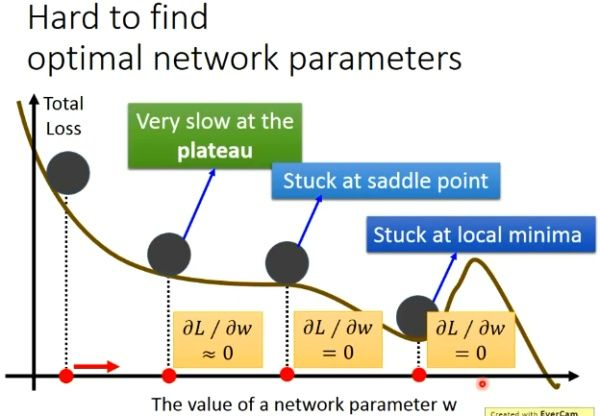
\includegraphics[width=0.7\textwidth]{sgd-momentum-01}

    \footnotehint{From: 李宏毅:机器学习}
  \end{center}
\end{frame}

\begin{frame}[fragile]
  \frametitle{动量梯度法的动机}

  \begin{center}
    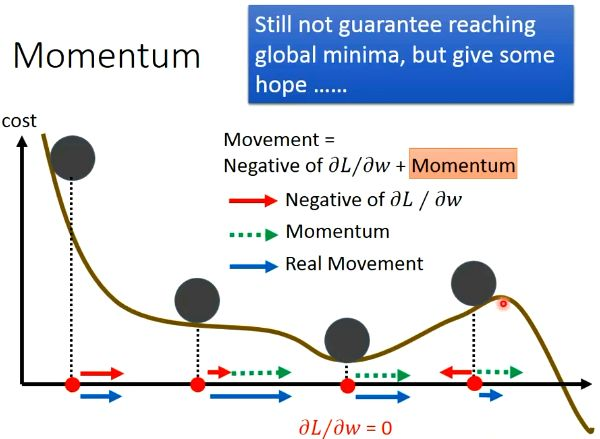
\includegraphics[width=0.7\textwidth]{sgd-momentum-03}

    \footnotehint{From: 李宏毅:机器学习}
  \end{center}
\end{frame}

\begin{frame}[fragile]
	\frametitle{动量梯度法 Gradient Methods with Momentum}
	动量梯度法是最速下降方向和最近迭代位移法的组合,这些方法的特点是迭代为
	\begin{equation} \tag{7.1}
		 w_{k+1} \leftarrow w_{k}-\alpha_{k} \nabla F\left(w_{k}\right)+\beta_{k}\left(w_{k}-w_{k-1}\right),
	\end{equation}
	右边的项被称为动量项.

    \begin{itemize}
    \item  当$\beta_k = 0$时, 对于所有 $k \in N$, 它简化为最速下降法.
    \item 当 $\alpha_k = \alpha > 0$ 且 $\beta_k = \beta > 0$ 时,对于所有  $k \in N$,  它被称为重球法(the heavy ball method).
  \end{itemize}
	
\end{frame}

\begin{frame}[fragile]
	\frametitle{动量梯度法 Gradient Methods with Momentum}
重球法的另一种观点是通过扩展 (7.1):
\begin{equation}\tag{7-1}
	w_{k+1} \leftarrow w_{k}-\alpha_{k} \nabla F\left(w_{k}\right)+\beta_{k}\left(w_{k}-w_{k-1}\right)
\end{equation}
$$
w_{k+1} \leftarrow w_{k}-\alpha \sum_{j=1}^{k} \beta^{k-j} \nabla F\left(w_{j}\right)
$$
这些步骤倾向于在持续下降的方向上积累贡献,而振荡的方向往往会被抵消,或者至少保持较小。

\end{frame}




\begin{frame}[fragile]
	\frametitle{加速梯度法Accelerated Gradient Methods}
	迭代类似于(7.1)的方法,但具有自己独特的性质,是涅斯捷罗夫(Nesterov)提出的加速梯度法.

$$
\tilde{w}_{k} \leftarrow w_{k}+\beta_{k}\left(w_{k}-w_{k-1}\right)
$$
$$
w_{k+1} \leftarrow \tilde{w}_{k}-\alpha_{k} \nabla F\left(\tilde{w}_{k}\right),
$$
从而形成缩合形式
\begin{equation}
	 \quad w_{k+1} \leftarrow w_{k}-\alpha_{k} \nabla F\left(w_{k}+\beta_{k}\left(w_{k}-w_{k-1}\right)\right)+\beta_{k}\left(w_{k}-w_{k-1}\right) .
\end{equation}

\end{frame}


%===========================================

\begin{frame}
{\textbf{总结}}


{\color{dblue}对比随机和Batch梯度方法}
$$\min\limits_{\mat{w}\in{\mathbb{R}^d}} F(\mat{w}):=\frac{1}{n}\sum\limits_{i=1}^{n}f_i(\mat{w})$$

{\color{blue}{最速下降算法}}
 $${ \mat{w}_{k+1} := \mat{w}_k - \frac{\alpha_k}{n}\sum_{i=1}^n\nabla f_i(\mat{w}_k)}$$
{\color{blue}{随机梯度算法}}
 $${ \mat{w}_{k+1} := \mat{w}_k - {\alpha_k} \nabla f_{i_k}(\mat{w}_{k})}$$
其中 $i_k$ 是从 $\{1,\cdots, n\}$随机选取的

{\color{blue}mini-batch SG}
 $$ {\mat{w}_{k+1}:=\mat{w}_k- \alpha_k \cdot \frac{1}{|S_k|}\sum\limits_{i\in S_k}\nabla f_i(\mat{w}_k)}$$

\end{frame}


\begin{frame}
{\textbf{总结}}


 { \color{dred}{SG方法的收敛性}}

\begin{itemize}
  \item 对于 FG, 如果 $F$ 是强凸函数, 那么
  $$F(\mat{w}_k) - F^*\leq \mathcal{O}(\rho^k), \text{线性收敛}$$
  其中 $\rho\in(0,1)$.
  求得 $\varepsilon$最优解所需的计算量与$n \log(\frac{1}{\varepsilon})$成正比.
%
  \item  对于 SG, 
   $$\mathbb{E}[F(\mat{w}_k) - F^*] =  \mathcal{O}(\frac{1}{k}), \text{次线性收敛} $$
求得 $\varepsilon$最优解所需的计算量与$\frac{1}{\varepsilon}$成正比.
\end{itemize}
\textbf{备注:}在大数据场景下, 对于$n$很大时, 有 $n \log(\frac{1}{\varepsilon}) > \frac{1}{\varepsilon}$.
\end{frame}


\begin{frame}
{\textbf{总结}}

\textbf{假设\,1}:
 $F$的梯度函数是Lipschitz连续的,
$\|\nabla F(w) - \nabla F(\overline w)\|_2\leq L\|w - \overline w\|_2 \,\, \,for \ all\,\, \{w, \overline{w} \}\subset \mathbb{R}^d.$

\bigskip 

\textbf{假设\,2}: 一阶矩和二阶矩假设

(a) $F$ 在开集上有下界;

(b)  $\exists\,\mu_G \geq \mu > 0$, $\forall\,k$
$$\nabla F(w_k)^T \mathbb{E}_{\xi_k}[g(w_k; \xi_k)] \geq \mu\|\nabla F(w_k)\|^2_2 \,\text{且}\,$$
$$\|\mathbb{E}_{\xi_k}[g(w_k; \xi_k)]\|_2\leq \mu_G\|\nabla F(w_k)\|_2.$$

(c)   $\exists\,M> 0, M_V \geq 0$, $\forall k$, $\mathbb{V}_{\xi_k}[g(w_k; \xi_k)] \leq M + M_V \|\nabla F(w_k)\|^2_2,$ \\
其中
$\mathbb{V}_{\xi_k}[g(w_k; \xi_k)] := \mathbb{E}_{\xi_k}[\|g(w_k; \xi_k)\|^2_2] - \|\mathbb{E}_{\xi_k}[g(w_k; \xi_k)]\|^2_2.$
 %

\end{frame}



\begin{frame}
{\textbf{总结}}


\begin{theorem}[强凸, 固定步长]
在假设 1 和 2成立的条件下, 假设 $F$ 是强凸的, SG方法的步长满足$\alpha_k = \bar{\alpha}$ 
$$ 0 < \bar \alpha\leq \frac{\mu}{L M_G},$$
那么,
$$\mathbb{E}[F(w_k)- F_*] \leq \frac{\bar\alpha L M}{2c\mu}+(1-\bar\alpha c \mu)^{k-1}
\left(F(w_1)-F_*-\frac{\bar\alpha L M}{2c\mu}\right).$$
\end{theorem}


\end{frame}


\begin{frame}
{\textbf{总结}}

 { \color{dred}{梯度聚合算法}}

是否通过重复使用或修改先前计算的信息来实现较低的方差?


\begin{itemize}
  \item SVRG (随机方差约减梯度)

  $$
  \tilde{{g}}_j \leftarrow \nabla f_{i_j}\left(\tilde{{w}}_j\right)-\left(\nabla f_{i_j}\left({w}_k\right)-\nabla R_n\left({w}_k\right)\right)
  $$
 
  \item SAGA(随机平均梯度算法)

$$
g_k \leftarrow \nabla f_j\left(w_k\right)-\nabla f_j\left(w_{[j]}\right)+\frac{1}{n} \sum_{i=1}^n \nabla f_i\left(w_{[i]}\right)
$$

\end{itemize}

\hint{梯度聚合方法 vs SG}
\begin{itemize}
  \item[-] SG 的计算时间为 $T(n, \epsilon) \sim \kappa^{2} / \epsilon$,
  其中 $\kappa:=L / c$
  \item[-] SVRG和SAGA 的计算时间为
  $\mathcal{T}(n, \epsilon) \sim(n+\kappa) \log (1 / \epsilon)$,
  随着样本点数量$n$的增加而增加
\end{itemize}

\end{frame}

\begin{frame}
{\textbf{总结}}

 { \color{dred}{其他流行优化算法}}

 \begin{itemize}
  \item Gradient Methods with Momentum 动量梯度法

 $$
\begin{array}{l}
\mathbf{v}_t=\gamma \mathbf{v}_{t-1}+\eta \nabla_\theta F(w) \\
\mathbf{w}_t=\mathbf{w}_t-\mathbf{v}_t
\end{array}
$$
  \item Accelerated Gradient Methods 加速梯度法
  
  $$
  \tilde{w}_{k} \leftarrow w_{k}+\beta_{k}\left(w_{k}-w_{k-1}\right)
  $$
  $$
  w_{k+1} \leftarrow \tilde{w}_{k}-\alpha_{k} \nabla F\left(\tilde{w}_{k}\right),
  $$
\end{itemize}
\end{frame}



\begin{frame}[fragile]
\frametitle{作业 }
\begin{itemize}

  \item[1.]编程实现 SVRG 和 SAGA 算法, 分别求解岭回归模型:
$$
\min _{\boldsymbol{w} \in \mathbf{R}^{\mathrm{d}}} \frac{1}{N} \sum_{i=1}^n\left(\boldsymbol{x}_i^{\top} \boldsymbol{w}-y_i\right)^2+\lambda \cdot \Omega(\boldsymbol{w})
$$
其中, $\left(\boldsymbol{x}_i, y_i\right) \in \mathbf{R}^d \times \mathbf{R}$ 为观测样本, $i=1, \cdots, n$, 正则化项 $\Omega(\boldsymbol{w})=\boldsymbol{w}^{\top} \boldsymbol{w}, \lambda>0$ 为给定的正则 化参数。

\end{itemize}
\end{frame}


\end{document}






